\documentclass[12pt,letterpaper]{article} %12-point font, US letter size
\usepackage{mathptmx} %Times new roman with math support
\usepackage{fontenc}
\usepackage[english]{babel}

\usepackage{amsmath,amssymb} %math support

%figures
\usepackage[pdftex]{graphicx} 
%\usepackage{epstopdf}

%bibliography
\usepackage{natbib} 
\bibliographystyle{evolution}

%colored hyperlinks
%\usepackage{hyperref}
%\usepackage[all]{hypcap}
%\hypersetup{
%     colorlinks   = true,
%     citecolor    = blue
%}
%\usepackage{color} %for notes to myself

%number pages
\usepackage{fancyhdr}
\pagestyle{fancy}
\pagenumbering{arabic}
\lhead{}
\rhead{\thepage}
%\cfoot{center of the footer!}
\renewcommand{\headrulewidth}{0pt}
%\renewcommand{\footrulewidth}{0pt}
%\fancyfoot[C]{}

%\usepackage{fullpage}
\usepackage{setspace} %double spacing
\usepackage{lineno} %line numbers

\begin{document}

%\newpage
%\thispagestyle{empty}
%\LARGE \MakeUppercase{An evolutionary tipping point in a changing environment}\\\vspace{0.5cm}
%%\LARGE \MakeUppercase{Selection as a constraint on adaptation and persistence in changing environments: an evolutionary tipping point}\\\vspace{0.5cm}
%%\LARGE \MakeUppercase{Selection as a constraint on adaptation and persistence in a changing environment}\\\vspace{0.5cm}
%%\LARGE \MakeUppercase{Selection as an evolutionary constraint: an evolutionary tipping point in a changing environment}\\\vspace{0.5cm}
%%\LARGE \MakeUppercase{Selection as an evolutionary constraint in changing environments}\\\vspace{0.5cm}
%\noindent\Large{\textbf{An evolutionary tipping point in a changing environment}} \vspace{0.5cm} %max 50 words
%
%\normalsize
%\noindent \textit{Running title:} Evolutionary tipping point \vspace{0.5cm} %max 50 characters
%
%%\noindent \textbf{Matthew Miles Osmond}\\
%%Biodiversity Research Centre \& Department of Zoology\\
%%University of British Columbia\\
%%6270 University Blvd. \\
%%Vancouver, BC V6T 1Z4, Canada\\
%%mmosmond@zoology.ubc.ca\\
%%Tel: 604 822 2131\\
%%
%%\noindent \textbf{Christopher A.\ Klausmeier}\\
%%Kellogg Biological Station \& Department of Plant Biology\\
%%Michigan State University\\
%%3700 East Gull Lake Drive\\
%%Hickory Corners, MI 49060, USA\\
%%klausme1@msu.edu\\
%%Tel:\\
%
%\noindent \textit{Keywords:} \textbf{Evolutionary rescue, extinction, fitness function, hysteresis, mathematical model, quantitative genetics}
%%max 6, not in title
%%Adaptation, s, moving optimum, rate of evolution, environmental change, tipping point
%
%\vspace{0.5cm}
%
%\noindent \textit{Word count:} 3291 (excluding Abstract, Acknowledgements, References, Figure Captions, Online Appendix)
%
%\noindent \textit{Table count:} \textbf{0}
%
%\noindent \textit{Figure count:} \textbf{4}

%\tableofcontents

\doublespacing
\linenumbers

%%%%%%%%%%%%%%%%%%%%%%%%%%%%%%%%%%%
%%%%%%%%%%%%%%%%%%%%%%%%%%%%%%%%%%%
\newpage
%\pagestyle{headings}
\setcounter{page}{1}
%\pagenumbering{arabic}
\pagestyle{fancy}

\noindent{\large{\textbf{An evolutionary tipping point in a changing environment}}}%max 50 words
\normalsize

\section*{Abstract} %max 200 words, currently 191

%Populations can persist in directionally changing environments by evolving as fast as the environment changes.
%Current theory predicts a critical rate of environmental change, beyond which a population is doomed to extinction.
%These predictions assume that selection on standing genetic variance of a quantitative trait becomes increasingly strong -- and therefore evolution proceeds increasingly fast -- as populations fall further from their optimal conditions.
%Hence, persistence is limited by demography only; the critical rate of environmental change is the rate at which population growth rate becomes zero.
%Here we analytically show that when the underlying fitness function does not allow infinitely strong selection, there exists a second, qualitatively different critical rate of environmental change.
%In particular, an upper bound on the strength of selection imposes a speed limit on adaptation.
%As the environment changes faster than this maximum rate the system undergoes a fold bifurcation.
%This bifurcation causes an \textit{evolutionary tipping point}, where a seemingly persistent population suddenly goes extinct.
%%If the environment changes faster than the maximum rate the population will quickly go extinct. %, regardless of population growth rate.
%We use simulations to corroborate our analytical treatment and examine the dynamics near the evolutionary tipping point.
%%Populations near this critical rate exhibit characteristic early warning signs of catastrophic transitions, providing cues of imminent extinction.
%We find that populations near their tipping point fail to exhibit characteristic early warning signs of imminent extinction and that the tipping point produces a type of evolutionary hysteresis that creates an extinction debt.
%The shape of the fitness function appears to have large implications in species persistence and extinction in our rapidly changing environments.
%The existence of the tipping point induces a type of \textit{evolutionary hysteresis}, or extinction debt, implying that future reductions in the rate of environmental change will not necessarily save populations from extinction, and that characteristic early warning signs do a poor job of signalling imminent extinction. 

Populations can persist in directionally changing environments by evolving. Quantitative genetic theory aims to predict critical rates of environmental change beyond which populations go extinct. Here we point out that all current predictions effectively assume the same specific fitness function. This function causes selection on the standing genetic variance of quantitative traits to become increasingly strong as mean trait values depart from their optima. Hence, there is no bound on the rate of evolution and persistence is determined by the critical rate of environmental change at which populations cease to grow. We then show that biologically-reasonable changes to the underlying fitness function can impose a qualitatively different extinction threshold. In particular, inflection points caused by weakening selection create local extrema in the strength of selection and thus in the rate of evolution. These extrema can produce evolutionary tipping points, where long-run population growth rates drop from positive to negative values without ever crossing zero. Generic early-warning signs of tipping points are found to have little power to detect imminent extinction, and require hard-to-gather data. Furthermore, we show how evolutionary tipping points produce evolutionary hysteresis, creating extinction debts. %Progress requires more empirically determined fitness functions as well as more robust and general theory.

%3-6 keywords
\noindent \textit{Keywords:} \textbf{Evolutionary rescue, extinction, fitness function, hysteresis, mathematical model, quantitative genetics}
%Keywords: \textbf{Absolute fitness, adaptation, catastrophe, environmental change, evolutionary constraints, extinction, fitness function, fold bifurcation, hysteresis, moving optimum, phase transition, quantitative genetics, rate of evolution, selection, tipping point}

\newpage
\section*{Introduction}

%Many populations are facing directional environmental change \citep[reviewed in][]{Davis2005,Parmesan2006,Visser2008,Lavergne2010,Hoffmann2011}.
%For example, migrating birds face earlier and earlier springs \citep[e.g.,][]{Nussey2005}, diapausing insects face increasing photoperiods \citep[e.g.,][]{Bradshaw2001}, and ectotherms face warming temperatures \citep[e.g.,][]{Huey2009}.
%%Dispersal and plasticity can help, but provide - at most - temporary persistence. 
%Dispersal and plasticity can help maintain adaptedness and prolong persistence \citep{Holt1990,Gienapp2008}, but long-term survival will likely require significant genetic adaptation.
%Genetic adaptation may be the ultimate solution.

%In a directionally changing environment populations can persist indefinitely by evolving as fast as the environment changes.
Many populations currently face gradual directional changes in their environment \citep[reviewed in][]{Davis2005,Parmesan2006,Visser2008,Lavergne2010,Hoffmann2011}.
Those populations with limited dispersal and plasticity can persist only if they evolve fast enough \citep{Lynch1993}.
The maximum rate of environmental change a population can adaptively track -- and demographically tolerate -- %is dubbed the `critical rate of environmental change' \citep{Lynch1991}. The critical rate of environmental change 
has recently received considerable theoretical attention \citep[reviewed in][]{Walters2012,Kopp2013,Alexander2014}. % and empirical  attention.
%The typical approach in quantitative genetics\footnote{Another mathematical approach to adaptation to directional environment change, but one which ignores the possibility of extinction, is the description of `traveling waves' \citep{Waxman1999,Rybka2003,Tang2003,Broom2003,Sato2008}. Interestingly, this is a direct equivalent of a problem in quantum theory \citep{Waxman2002}.} is essentially as follows: set the rate of evolution of population mean phenotypic lag value $\frac{d}{dt}\bar{z}$ equal to the rate of change of the environmentally determined optimal phenotypic lag value $\frac{d}{dt}z_{opt}$ and solve for the mean phenotypic lag $z_{opt}-\bar{z}$.

Typically these studies follow a quantitative genetic approach \citep[for alternatives see][]{Johansson2008,Bertram2016,Osmond2017}.
They first assume some unimodal mapping from phenotype to absolute fitness (the `fitness function').
%Next one calculates the expected phenotypic lag of the population mean phenotype behind the changing optimum.
%If the phenotypic lag is too large the population has a negative growth rate and is predicted to perish, while if the phenotypic lag is small enough to permit positive growth rate the population is predicted to persist.
Then, for a given rate of change in the trait value that maximizes fitness (the `environmental optimum'), the fitness function is used to derive the rate of evolution in the mean trait value and the expected difference between the mean trait value and the optimum at equilibrium (the `steady-state lag').
The rate of environmental change that produces a steady-state lag resulting in a population mean growth rate (when rare) of zero is dubbed the `critical rate of environmental change' \citep[][]{Lynch1991}.
%(or, with density-dependent growth, an equilibrium population size of zero; Osmond \textit{et al}.\ 2017)
%\citep{Pease1989,Lynch1991,Lynch1993,Burger1995,Lande1996,Burger1997}
Critical rates of environmental change are now being estimated and used to predict whether particular species will survive or go extinct in the face of global climate change \citep{Aitken2008,Willi2009,Gienapp2013,Vedder2013}.

To the best of our knowledge, all quantitative genetic theory developed so far implicitly assumes that the maximum rate of environmental change to which a population can adapt is determined by demography (i.e., `selective load' \textit{sensu} \citealt{Lynch1993}, or `demographic constraint' \textit{sensu} \citealt{Gomulkiewicz2009}). 
This assumption results from the shape of the specific fitness functions used.
In particular, Gaussian fitness functions, $W(z)$, are used in models with non-overlapping generations in discrete time \citep{Charlesworth1993c,Burger1995,Burger1997,Burger1999a,Gomulkiewicz2009,Chevin2010,Matuszewski2015,Marshall2016}, while quadratic fitness functions, $r(z)$, are used in models with overlapping generations in continuous time \citep{Pease1989,Lynch1991,Lynch1993,Polechova2009,Aguilee2016}.
These are equivalent given $\log(W)=r$ \citep[][Chapter 1]{Crow1970} and have presumably been chosen for mathematical convenience (e.g., they maintain a normal trait distribution) as well as their ability to approximate -- when near the optimum -- any smooth fitness function imposing stabilizing selection \citep[][]{Lande1976}.
This particular fitness function is therefore a relatively mild assumption under the historical paradigm of weak selection, but it becomes a strong yet biologically arbitrary assumption when environments change quickly enough that populations find themselves considerably maladapted.

The rate of evolution in a mean trait value can be approximated by the product of additive genetic variance and the selection gradient \citep[][]{Lande1976}.
With overlapping generations in continuous time, the selection gradient is the derivative of mean fitness with respect to mean trait value \citep[][equation 11]{Lande1982b}, while with non-overlapping generations in discrete time, it is the derivative of the logarithm of mean fitness \citep[][equation 7]{Lande1976}. %while in continuous time weak selection means that Gaussian fitness functions can be approximated by quadratics.
%Models in continuous time that do not explicitly assume weak selection begin with quadratic fitness functions \citep{Pease1989,Polechova2009,Aguilee2016}.
%Since calculating the rate of evolution in discrete time involves the natural logarithm of fitness \citep[e.g., equation 7 in][]{Lande1976}, the Gaussian fitness functions used there are effectively reduced to quadratics.
%The result of such `effectively quadratic' fitness functions is a rate of evolution that increases linearly with phenotypic lag. %(assuming constant genetic variance; see \cite{Polechova2009} for theoretical support of constant genetic variance).
%This resulting in a rate of evolution that increases linearly with phenotypic lag. %(assuming constant genetic variance; see \cite{Polechova2009} for theoretical support of constant genetic variance).
%In other words, selection can become infinitely strong and the optimal phenotypic lag value is always an evolutionary attractor; the limiting factor determining population persistence is mean growth rate at the phenotypic lag that produces the necessary rate of evolution.
%Thus the rate of evolution becomes a quadratic function of phenotypic lag in all models listed above.
%This allows selection to become infinitely strong and adaptation to proceed infinitely fast as lag increases.
%%Quadratic fitness functions allow selection to become infinitely strong and adaptation to proceed infinitely fast as lag increases.
%Mathematically, there is always a phenotype that is an evolutionary attractor; the limiting factor determining population persistence is mean growth rate at the phenotypic lag that produces the necessary rate of evolution. %(Box 1).
%Thus, these landscapes ensure the limiting factor in the potential rate of evolution is the population growth rate.
Thus the strength of selection becomes a linear function of mean phenotypic lag in all models listed above. %\citep[a notable exception comes from the adaptive dynamics literature, where the lack of phenotypic variance allows greater freedom of choice in fitness functions without sacrifices in analytic tractability;][]{Johansson2008}.
%This implies that selection can become infinitely strong and therefore that the rate of evolution can become infinitely fast (as long as additive genetic variance remains non-zero), meaning there is always a steady-state lag that is an evolutionary attractor. 
This implies that the strength of selection has no limit and therefore that, given a large enough steady-state lag, evolution can proceed arbitrarily fast (as long as additive genetic variance remains non-zero).
Population persistence is then only determined by the population mean growth rate at the steady-state lag that causes evolution to proceed as fast as the environment changes, i.e., there is a critical rate of environmental change at which populations cease to grow.

%The use of unbounded unimodal fitness functions (e.g., quadratic fitness functions in continuous time) %(as used in previous analyses of overlapping generations in continuous time) 
%is not always justified. 
%%First of all, there is no biological reason why fitness functions should be different in continuous \textit{vs}.\ discrete time; quadratic fitness functions are used solely for mathematical convenience.
%First, an unbounded unimodal fitness function implies the process which depends on phenotype can take on negative values when the phenotypic lag is large.
%This is clearly unrealistic when the phenotype-dependent rate is the birth rate, which must be strictly non-negative.
%Second, intuitively one might expect that when a population is sufficiently maladapted, individual variants slightly closer to the optimum phenotype may have very little adaptive advantage.
%This suggests a fitness function which becomes flatter (i.e., bounded and unimodal, e.g., Gaussian), not steeper (which occurs with a quadratic fitness function), as the phenotypic lag becomes large.
%A fitness function mathematically derived from energetic principles and allometry supports this intuition \citep{Brown1993}.  
%Finally, numerous studies provide empirical support for bounded unimodal fitness functions, at least in one phenotypic direction \cite[e.g.,][]{Schluter1988,Weis1992,Schluter1994,Martin2006,Rokyta2011,VanValen1967}.

%Here we compare two extreme fitness functions: a quadratic (unbounded unimodal), which allows evolution to occur infinitely fast as phenotypic lag increases, and a Gaussian (bounded unimodal), which assumes the rate of evolution approaches zero as lag increases.
Here we show that the existence of a critical rate of environmental change depends on the choice of fitness function. 
%In particular, if selection cannot become infinitely strong there exists a maximum rate of evolution.
%compare how adaptation and persistence depend on the rate of environmental change with two alternative fitness functions: a quadratic (unbounded unimodal), which allows evolution to occur infinitely fast as phenotypic lag increases, and a Gaussian (bounded unimodal), which assumes the rate of evolution approaches zero as lag increases.
%In doing so, we highlight an important consequence of bounded unimodal fitness functions in determining a population's fate in the face of a changing environment: there exists a finite phenotypic lag which maximizes the rate of evolution.
%If the population can persist at the phenotypic lag that causes this maximum rate of evolution there is no critical rate of environmental change, as defined above.
Moreover, decreases in the strength of selection (the slope of the fitness function) with increasing maladaptation cause local maxima in the rate of evolution.
These local maxima can create an `evolutionary tipping point', where rates of environmental change less than the tipping point result in stable steady-state lags and population persistence while rates of environmental change greater than the tipping point lead to an apparent existential crisis: the population ceases to adapt as the selective pressure relaxes, causing the steady-state lag to rapidly increase and the population to go extinct. 
%Instead, the relevant persistence metric is the maximum rate of evolution.
%We call the maximum rate of evolution an `evolutionary tipping point' as rates of environmental change less than the maximum result in stable steady-state lags and population persistence while rates of environmental change greater than the maximum cause an ``existential crisis": the population ceases to adapt as the selective pressure relaxes, causing the lag to tend to infinity and the population to go extinct. %(i.e., the system undergoes a saddle-node bifurcation as the rate of environmental change moves through the evolutionary tipping point). %produce phenotypic lags that tend toward infinity (i.e., the system undergoes a fold bifurcation as the rate of environmental change moves through the evolutionary tipping point).  
%After a general treatment we demonstrate the result in an explicit ecological context (temperature- and phenotypic lag-dependent birth rate in phytoplankton in a warming lake).
%mention ecological "tipping points" (eg Carpenter)
This existential crisis is brought about by what is known as a saddle-node bifurcation.
Many dynamical systems are thought to experience saddle-node bifurcations, from global finance to climate, and there is a substantial literature devoted to developing generic early-warning signs to detect impending bifurcations \citep[reviewed in][]{Scheffer2009}.
Two common early-warning signs are increased variance and lag-1 autocorrelation, both of which are caused by slow recovery from perturbation, or a `critical slowing down', and have been detected in climate and ecological data \citep{Scheffer2009,Lenton2011}.
We therefore use simulations to see if generic early-warning signs have the potential to detect evolutionary tipping points, granted one has extensive time series of difficult-to-measure parameters such as mean phenotypic lag.
Finally, we show how the existence of an evolutionary tipping point induces `evolutionary hysteresis', which can create an extinction debt: transitory increases in mean phenotypic lags (e.g., due to sudden environmental changes) can initiate the above mentioned existential crisis, with extinction occurring many generations later even if the rate of environmental change returns to moderate levels.
Overall, our results demonstrate that our current understanding of evolutionary rescue in directionally changing environments is highly sensitive to the -- relatively unknown -- shape of fitness functions as populations become increasingly maladapted.

\section*{Methods and Results}
\subsection*{A general model}

%Now that we have defined what we mean by  a bounded unimodal function, let us examine the effect a bounded unimodal fitness function has on the predicted rate of evolution.
%Let us now examine how the shape of the fitness function affects the predicted evolutionary dynamics.
Following \cite{Lynch1993}, we consider a well-mixed and randomly mating population of short-lived, hermaphroditic individuals with overlapping generations in continuous time.
%The dynamics of population density $N$ are described by $dN/dt=r(z)N$, where $r(z)$ is the intrinsic growth rate for individuals with phenotype $z$.
%This implies that $r(z)$ is the appropriate fitness function \citep{Lande1976}.
%Let $b(z)$ be the birth rate and $d(z)$ be the death rate of individuals with quantitative trait $z$ and define the trait-specific growth rate $r(z) = b(z) - d(z)$. 
Individuals are characterized by a quantitative trait, $z$, which is the sum of genetic and environmental effects, $z = g + e$.
The genetic effect is determined by a large number of equivalent, additive, and freely-recombining diploid loci.
The environmental effect is an independent random normal variable with mean 0 and variance $\sigma_e^2$.
%We set $\sigma_e^2=1$ such that trait values are scaled by their environmental variance \citep{Burger1995}.
The population mean trait value is then the mean genetic effect, $\bar{z} = \bar{g}$, while the phenotypic variance is the sum of additive genetic and environmental variance, $\sigma_z^2 = \sigma_g^2 + \sigma_e^2$.

%And let $p(z)$ be the distribution of trait values in the population.
%Note that density-dependence can easily be included \citep{Lande1996}, but is omitted here for clarity and comparison to classic results \citep[e.g.,][]{Lynch1991}.
%We decompose intrinsic growth rate into birth and death terms, and assume, for simplicity, that stabilizing selection occurs only through births and death does not depend on phenotype, $r(z)=b(z)-d$.
%The population mean growth rate is then $\bar{r} = \int r(z) p(z) \mathrm{d}z$.
%The population is growing if $\bar{r} > 0$ and declining if $\bar{r} < 0$.

Ignoring frequency-dependence for simplicity, let $r(z)$ be the per capita growth rate when rare (hereafter fitness) of individuals with quantitative trait $z$.
Let density-dependence affect all individuals equally.
The expected rate of change in the current mean trait value due to natural selection on standing genetic variation is then approximately the product of standing genetic variance and the selection gradient, $\mathrm{E}[\mathrm{d}\bar{z}/\mathrm{d}t] = \mathrm{d}\bar{g}/\mathrm{d}t \approx \sigma_g^2 \partial \bar{r} / \partial \bar{g}$, where $\bar{r}$ is the population mean growth rate.
We assume additive genetic variance remains constant at some equilibrium (which we estimate in specific examples below and compare to simulations).

Now assume there is some trait value, $\theta$, that maximizes fitness, $r(z)$, and let this value increase linearly in time at rate $k$, such that its value at time $t$  is $\theta(t) = k t$. % + \epsilon_\theta$ where $\epsilon_\theta$ describes stochasticity in the environment.
%We assume that the value of $\epsilon_\theta$ at any time $t$ can be reasonably described by a random normal variable with mean 0 and variance $\sigma_\theta^2$, such that there is no correlation between values of $\epsilon_\theta$ across time \citep[][equation 3]{Lynch1993}.
%\subsection*{A critical rate of environmental change may not exist}
A quasi-steady-state is then achieved when the expected rate of evolution matches the rate of change in the environment, $\mathrm{d}\bar{g}/\mathrm{d}t = k$.
%This gives an equation for the steady-state lag $\hat{L} = \theta - \bar{z}$.
If at this steady-state the expected population mean growth rate is positive, $\bar{r} > 0$, the population will persist.
If instead the growth rate is negative, $\bar{r} < 0$, the rate of environmental change is too fast and the population goes extinct.
The rate of environmental change that causes an expected growth rate of zero, $\bar{r} =0$, at steady-state is termed the critical rate of environmental change, $k_c$. 

However, there is also the -- yet to be discussed -- possibility that such a steady-state does not exist.
%This is a fact that has been so far overlooked \citep[but see][]{Osmond2017}.
In particular, a steady-state does not exist if the rate of evolution has some maximum and the rate of environmental change is beyond this.
%With constant additive genetic variance the rate of evolution has some maximum when there exists a real-valued $z^*$ such that $0 = \frac{\mathrm{d}}{\mathrm{d}\bar{z}} (\mathrm{d}\bar{r}/\mathrm{d}t)_{\bar{z} = z^*}$ and $0 > \frac{\mathrm{d}^2}{\mathrm{d}\bar{z}^2} (\mathrm{d}\bar{r}/\mathrm{d}t)_{\bar{z} = z^*}$.
%If the population cannot persist at the lag that causes the maximum rate of evolution ($\bar{z} = z^*$ causes $\bar{r} < 0$) then the maximum rate of evolution is of no consequence and the critical rate $k_c$ is the meaningful measure of persistence ability.
%Population growth rates will then steadily decline to zero as $k$ approaches $k_c$.
More importantly, if, over the range of phenotypic lags that allow population persistence, 
%$L\equiv\theta-\bar{z}\in [0,L_{c})$ where $\bar{r}|_{\bar{z} = \theta - L_c} = 0$, 
the rate of evolution is maximal at some intermediate lag, 
%, $L^* < L_{c}$, 
then population growth rate at steady-state will not decline continuously towards zero as the rate of environmental change increases (see supplementary online material for a more technical discussion).
%If the population can persist ($\bar{r} > 0$ at $\bar{z} = z^*$), then the maximum rate of evolution, $k_{tip} = (\mathrm{d}\bar{z}/\mathrm{d}t)_{\bar{z}=z^*}$, is the meaningful measure of persistence ability.
%This means that a population can be growing quickly when rates of environmental change are less than the maximum rate of evolution, $k < k_{tip}$, and suddenly go extinct when $k_{tip} < k$.
%
Instead, the long-run population growth rate will jump from a potentially large positive number to a potentially very negative number as the rate of environmental change increases through the maximum rate of evolution.
Technically, this is due to an inflection point in the fitness function causing a saddle-node bifurcation.
When this bifurcation causes extinction we refer to the maximum rate of evolution as an `evolutionary tipping point'. %,  $k_{tip}\equiv\mathrm{d}\bar{z}/\mathrm{d}t\big|_{L=L^*}$.
%A maximum rate of evolution has also been found\citep[a notable exception comes from the adaptive dynamics literature, where the lack of phenotypic variance allows more freedom of choice in the fitness function without sacrifices in analytic tractability;][but in this case intrinsic growth rates cannot become negative and hence the maximum rate of evolution is the only possible persistence criterion]{Johansson2008}.
%Because rates of evolution are proportional to the slope of mean fitness with respect to mean trait value, local minima and maxima in the rate of evolution, and thus evolutionary tipping points, can be created by inflection points in the fitness function, which can occur even if the fitness function is unimodal.
When an evolutionary tipping point exists it is the meaningful predictor of persistence (disregarding stochastic factors), and there is no critical rate of environmental change as defined by \cite{Lynch1993}.

%  $k=\mathrm{d}\bar{z}/\mathrm{d}t\big_{$L=L^*$}$
%In other words, extinction is caused by a saddle-node bifurcation in the steady-state lag as the rate of environmental change increases through the maximum rate of evolution, and thus we refer to the maximum rate of evolution as an evolutionary tipping point,  $k_{tip}\equiv\mathrm{d}\bar{z}/\mathrm{d}t\big|_{L=L^*}$.

To demonstrate the effect of changes in the shape of the commonly assumed fitness function more concretely, we will next compare results arising from the `traditional' fitness function to those arising from an alternative fitness function that imposes a limit on the rate of evolution (see the supplementary material for detailed derivations).
In doing so we do not mean to imply that our alternative fitness function is necessarily always more biologically relevant than the traditional.
%In particular, it is not the case that evolutionary tipping points require Malthusian fitness, $r(z)$, to be bounded below, but only that they must have at least one inflection point.
Our alternative fitness function is used only to demonstrate that subtle changes in the shape of the fitness function may have dramatic effects on our predictions for adaptation and persistence in a rapidly changing world.

%To summarize, persistence is determined by an evolutionary tipping point $k_{tip}$ when there exists a real-valued $z^*$ such that
%\begin{enumerate}
%\item $0 = \frac{\mathrm{d}^2}{\mathrm{d}\bar{z}^2} \bar{r}\big|_{\bar{z} = z^*}$
%\item $0 > \frac{\mathrm{d}^3}{\mathrm{d}\bar{z}^3} \bar{r}\big|_{\bar{z} = z^*}$
%\item $0 < \bar{r}\big|_{\bar{z} = z^*}$
%\end{enumerate}
%where we've used Lande's (\citeyear{Lande1976}) approximation for the rate of evolution in the mean trait value assuming the presence of some positive amount of additive genetic variance, $V_A>0$.
%In words, points (1) and (2) say that there is a change in the curvature of mean growth rate $\bar{r}$ from convex to concave as the mean trait value $\bar{z}$ increases through the inflection $z^*$ and point (3) says that the population should be able to persist at $\bar{z} = z^*$.
%We next compare results arising from the traditionally used growth rate function (which does not satisfy 1 or 2) to those arising from a growth rate function that satisfies the above three conditions.

%We will compare results arising from a Gaussian (bounded unimodal) fitness function
%\begin{equation}\label{Gauss}
%r(z) = b_{max} \exp \left[-\frac{\gamma}{2} \left( \theta - z \right)^2\right] - d
%\end{equation}
%with those arising from its quadratic (unbounded unimodal) approximation, similar to that used in previous analyses of the problem \citep[e.g.,][]{Lynch1991},
%\begin{equation}\label{Quad} 
%r(z) = b_{max} \left[ 1 - \frac{\gamma}{2} \left(\theta - z \right)^2 \right] - d.
%\end{equation}
%Here $b_{max}$ is the maximum per capita birth rate, achieved by individuals with the optimum phenotype $z = \theta$, $d$ is the constant per capita death rate, and $\gamma$ is the strength of stabilizing selection. %(Figure \ref{Evolution}).
%Similar results can be obtained when allowing death, $d$, to also depend on phenotype; the essential element is that Equation \eqref{Gauss} does not become infinitely steep in $z$ while Equation \eqref{Quad} does.

\subsection*{The traditional fitness function}

%Let us begin with the traditionally used quadratic fitness function, $r(z) = b_{max} \left[ 1 - \frac{\gamma}{2} \left(\theta - z \right)^2 \right] - d$. 
%This is equation 1 in \cite{Lynch1993} with maximum growth rate $r_m = b_{max} - d$ and selection strength $\sigma_w^{-2} = b_{max} \gamma$.
%The population mean growth rate is then $\bar{r} = b_{max} \left( 1 - \frac{\gamma}{2} \left[ \left( \theta - \bar{z} \right)^2 - V_z \right] \right) - d$.
%Mean growth rate is depressed by phenotypic lag $|\theta - \bar{z}|$ as well as phenotypic variance $V_z$.
%%Persistence requires a positive mean growth rate, $\bar{r}>0$.
%
%%Note that the phenotype can be written as the sum of genetic and environmental components $z=g+e$, which have respective variances, $V_g$ and $V_e$ \citep[e.g.,][]{Lynch1991}.
%%Here we assume no environmental effect on phenotype, and hence $\bar{z} = \bar{g}$ and $V_z = V_g$. 
%%Including environmental variance depresses the mean population growth rate, by an additional amount $V_e\gamma/2 $, but has no qualitative effect and is therefore omitted for simplicity. 
%%Meanwhile, our simulations make use of the decomposition as it provides a logical way of calculating the expected equilibrium phenotypic variance (see below).   
%
%With constant genetic variance $V_g$ the rate of evolution is \citep{Lande1976}
%\begin{equation}\label{EvoQ}
%\frac{\mathrm{d}\bar{z}}{\mathrm{d}t} = V_g \frac{\partial \bar{r}}{\partial \bar{z}}
%% = b_{max} \frac{\sigma_g^2(z_{opt}-\bar{z})}{\sigma_w^2}.
%\end{equation}
%Note that increasing the phenotypic lag always increases the rate of evolution.
%In the supplementary \texttt{Mathematica} file we derive the rate of evolution and the equilibrium additive genetic variance using the infinitesimal model \citep{}.
%The analysis assumes a large (but finite) population, random mating, and offspring that inherit the average of the two parental trait values plus a small normally distributed random effect with mean zero and variance $\alpha^2$ (which mimics segregation and recombination).
%The rate of evolution is then $\frac{\mathrm{d}\bar{z}}{\mathrm{d}t} \approx \frac{V_z}{2} b_{max} \gamma (\theta - \bar{z})$ aligning with \cite{Lande1976} with additive genetic variance $V_g = V_z/2$ (the phenotypic variance is halved because the parent selected to give birth randomly mates, and the offspring inherits the average trait value).
%Equation \eqref{EvoQ} shows that increasing maladaptation, $|\theta-\bar{z}|$, linearly increases the (absolute) rate of evolution, so that there is no maximum evolutionary rate.
%
%When the variance introduced at each birth is small, $\alpha << 1$, additive genetic variance reaches an equilibrium between the variance introduced at birth and that lost due to random mating, $\hat{V}_g \approx \alpha^2$ (see supplementary \texttt{Mathematica} file).
%Our analytical and numerical approximations will assume that additive genetic variance is constant at this equilibrium.
%These assumptions are checked with stochastic individual-based simulations in which the variance is free to evolve.

We begin with the traditional fitness function in continuous time,  $r(z) = r_m - (\theta - z)^2 / (2\sigma_w^2)$ \citep[][equation 1]{Lynch1993}, where $r_m$ is the maximum per capita growth rate and $\sigma_w^2$ determines the strength of stabilizing selection (stronger if smaller) around $\theta$.
Averaging over the phenotypic distribution, we find that population mean growth rate, $\bar{r}$, is reduced by the magnitude of the mean phenotypic lag, $\bar{l} = \theta - \bar{z} $, and by standing genetic variance \citep{Lande1996}, e.g., when the mean trait value matches the optimum, $\bar{l}=0$, the mean growth rate is $\bar{r}_m = r_m - \sigma_z^2/(2\sigma_w^2)$.
Furthermore, this function implies that as mean trait value departs from the optimum population growth rate declines ever more rapidly, and there is no bound on how negative it can become (gray curve in Figure \ref{SSGrowth}A).

%Assuming the distribution of phenotypes can be transformed such that it is normally distributed, the population mean growth rate is $\bar{r}(\bar{g}) = r_m - (\theta - \bar{g})^2 / (2\sigma_w^2) - \sigma_z^2/(2\sigma_w^2)$ \citep[][equation 2]{Lynch1993}.
%Here we have assumed the quantitative trait $z$ is the sum of an additive genetic component, $g$, and an environmental component, $e$ (i.e., no dominance or epistasis).
%The additive genetic component is determined by the sum of the effects at $n$ freely-recombining diploid loci, and has population mean $\bar{g}$ and variance $\sigma_g^2$.
%We assume a continuum of alleles \citep{}.
%The environmental component is a random normal variable with mean 0 and variance $\sigma_e^2$.
%The total amount of phenotypic variance is then the sum of additive genetic variance and the environmental variance, $\sigma_z^2 = \sigma_g^2 + \sigma_e^2$. 

The expected rate of evolution given the current mean genotypic value is $\mathrm{d}\bar{g}/\mathrm{d}t = \sigma_g^2 (\theta - \bar{g}) / \sigma_w^2$ \citep[][equation 5]{Lynch1993}.
This is a linear function of the expected mean phenotypic lag, $\mathrm{E}[\bar{l}] = \theta - \bar{g}$, and therefore as lag increases so too does the rate of evolution, without bound (gray curve in Figure \ref{SSGrowth}B).
Thus, there is always a solution to the quasi-steady-state equation $\mathrm{d}\bar{g}/\mathrm{d}t  = k$, i.e., there is always some expected mean lag, $\mathrm{E}[\bar{l}]=\hat{l}$, that produces the required rate of evolution. %, and hence there is always a steady-state lag.

In this particular case the steady-state lag is $\hat{l} = k \sigma_w^2/\sigma_g^2$ (gray curve in Figure \ref{SSGrowth}C).
Evaluating the population mean growth rate at this lag gives the expected long-run population growth rate for an infinitely large population in a deterministic environment.
Increasing rates of environmental change cause a smooth decline in this long-run growth rate (gray curve in Figure \ref{SSGrowth}D).
We can therefore solve for the rate of environmental change, $k$, that makes the long-run growth rate 0, giving the critical rate of environmental change, $k_c = \sigma_g^2 \sqrt{2\bar{r}_m/\sigma_w^2}$ \citep[][equation 11]{Lynch1993}.

\subsection*{An alternative fitness function}

Here we alter the assumption that fitness declines increasingly fast as trait values depart from the optimum. %and that fitness can become infinitely negative.
Instead, we depict a scenario where, far from the optimum, small departures from the optimum have smaller and smaller fitness consequences.
This could result from selection becoming weaker with increasing maladaptation \citep[for which there is some evidence;][]{Agrawal2010}, which in turn could be caused by a lower bound on fitness (i.e., there is some maximum rate at which a population can decline).
For example, when selection acts only through birth rate, which cannot be negative, while death rate ($m>0$) is fixed, Malthusian fitness is bounded below by $-m$.
However, we would like to emphasize that growth rates do not have to be bounded below for evolutionary tipping points to exist -- all that is required is an inflection point.

Consider an alternative fitness function $r(z) = r_m - d\left[1 - \exp\left(-(\theta-z)^2/(2\sigma_w^2)\right)\right]$.
This is a Gaussian fitness function (in \textit{continuous} time) with maximum growth rate $r_m$ at $z=\theta$ and minimum growth rate $r_m-d$, achieved as lags tend to plus or minus infinity.
For comparison, the alternative fitness function has been constructed such that when $d=1$ it is equivalent to the traditional fitness function, to second order, when trait values are near the optimum.
Averaging over the phenotypic distribution, we find that the population mean growth rate (black curve in Figure \ref{SSGrowth}A) has an inflection point at mean lag $\mathrm{E}[\bar{l}] = V^{1/2}$, where $V = \sigma_w^2 + \sigma_z^2 + \sigma_\theta^2$.

The expected rate of evolution is $\mathrm{d}\bar{g}/\mathrm{d}t  = d\sigma_g^2 \sigma_w \mathrm{E}[\bar{l}] \exp\left[ -\mathrm{E}[\bar{l}]^2 / (2V) \right] / V^{3/2}$ (black curve in Figure \ref{SSGrowth}B).
The rate of evolution is no longer a linear function of expected mean lag, $\mathrm{E}[\bar{l}]$.
Instead, there is a maximum rate of evolution, $k_{tip} = d \sigma_g^2 \sigma_w \exp(2)/V$, at the inflection point, $\mathrm{E}[\bar{l}] = V^{1/2}$.

When the rate of environmental change is less than this maximum rate of evolution, $k<k_{tip}$, the steady-state lag is $\hat{l} = (V w_k)^{1/2}$ (solid black curve in Figure \ref{SSGrowth}C), where $w_k$ is the solution to $w_k e^{w_k} = (k V)^2 / (d\sigma_g^2\sigma_w)^2$ \citep[i.e., $w_k(x)$ is the Lambert W function, and here $x=(k V)^2 / (d\sigma_g^2\sigma_w)^2$;][]{Lehtonen2016}.
If this lag remains biologically valid (real) at the point where the expected long-run population growth rate becomes zero, there is a critical rate of environmental change, $k_c$, that determines persistence. %, $k_c = \sigma_g^2 \sigma_w (y^{2(\sigma_w^2+\sigma_z^2)/V} (\sigma_w^2+\sigma_z^2) \log(y))^{1/2} / V^{3/2}$, where $y = (1 - r_m) (\sigma_w^2 + \sigma_z^2)^{1/2}/\sigma_w$.
%This steady-state lag is a valid solution (i.e., a real number) only when $k < 
If, on the other hand, there is no valid steady-state lag that gives a population growth rate of zero then there is no `critical rate of environmental change', as typically defined \citep{Lynch1993}.
Instead, it is the maximum rate of evolution that determines persistence (with weak selection this occurs when $d[1-\exp(-1/2)]<r_m<d$; the upper bound is required to ensure the population goes extinct as lag tends to infinity), and the maximum rate of evolution is an `evolutionary tipping point' (black curves in Figure \ref{SSGrowth}D).
%In this case, as the rate of environmental change increases through the maximum rate of evolution the steady-state lag undergoes a saddle-node bifurcation; the steady-state lag, which allowed population persistence, disappears and the mean lag is expected to increase rapidly without bound, causing extinction.
%For this reason we say there is an evolutionary tipping point when the maximum rate of evolution determines persistence.

When the rate of environmental change is less than the maximum rate of evolution the population mean growth rate is $\bar{r} = r_m - \left[ 1 - \sigma_w \exp\left( - \hat{l} / (2(\sigma_w^2 + \sigma_z)^2) \right)\right] > 0$. 
This can be substantially positive right up to the tipping point (where $\hat{l} = V^{1/2}$) when the maximum growth rate is large, $r_m\approx d$. %, selection is weak (i.e., $\sigma_w^2$ is large), and there is little phenotypic or environmental variance (recall that phenotypic variance depends on additive genetic variance, which can be a function of many parameters including the strength of selection).
However, as soon as the rate of environmental change increases above the maximum rate of evolution, the mean lag increases quickly without bound, leading to a population growth rate of $\bar{r} \approx r_m - d$, and therefore rapid extinction when the maximum population growth rate is small, $r_m << d$.
In any case, at the evolutionary tipping point, long-run population growth rates go from positive values to negative values without ever crossing zero, causing what may appear to be highly sustainable populations to rapidly begin to go extinct.
%This swing in growth rates can be particularly dramatic when selection is weak and there is little phenotypic or environmental variance (Figure \ref{SSGrowth}B).

\subsection*{Simulations}

We next use stochastic, individual-based simulations to (\textit{i}) compare the dynamics arising from the traditional and alternative fitness functions, (\textit{ii}) examine generic early-warning signs of approaching tipping points, and (\textit{iii}) demonstrate the consequences of evolutionary hysteresis.

\subsubsection*{Simulation methods}

We use discrete time simulations with non-overlapping generations \citep[as described in][]{Burger1995}, which allows us to compare our results to previous studies and provides us with analytical predictions for the additive genetic variance \citep[equations 14 and 15 in][]{Burger1995} as well as empirically justified parameters \citep{Burger1995}.
To convert our continuous time models into discrete time, we set the expected number of offspring per parent to $B=\exp(r_m)$ and the probability of survival to adulthood $W(z)=\exp[r(z)-r_m]$, such that growth rates in the absence of density-dependence are equivalent, $BW(z)=\exp[r(z)]$ \citep[][Chapter 1]{Crow1970}.
Example scripts (Python Software Foundation, version 3.5; http://www.python.org) are provided in the supplementary material.

Briefly, each individual's trait is determined by $n$ additive, freely-recombining diploid loci plus a random normal environmental effect with mean 0 and variance 1.
All simulations are initiated as in \cite{Burger1995}; we create 5 ancestral alleles at each locus, their effects being random normal variables with mean 0 and variance $(0.1\alpha)^2$. %change to 4Ne n mu alpha^2?
The first generation of individuals are then created by randomly choosing two ancestral alleles for each locus, with replacement.
Simple density dependence then acts by randomly choosing $K$ individuals if there are more than $K$.
These pair at random (potentially leaving one individual out) and each pair produces 2$B$ offspring by fair Mendelian transmission.
Each gamete mutates with probability $n \mu$.
If it does mutate one locus is chosen at random and a random normal effect, with mean 0 and variance $\alpha^2$, is added.
Viability selection then acts, with survival probability $W(z)$.
A maximum $K$ surviving offspring become the parents of the next generation.
The first 1,000 generations are used as a burn-in with $k=0$.
Simulations continue until the population goes extinct or the maximum number of generations is reached (11,000 in Figures \ref{ModerateSummaryLast} and \ref{HysteresisSnapshot}; 201,000 in Figure \ref{ModerateWarnings}).

\subsubsection*{Comparing the dynamics arising from traditional and alternative fitness functions}

Figure \ref{ModerateSummaryLast} shows the effect of the rate of environmental change on evolution and persistence with the traditional (A-E) and alternative fitness functions (F-J).
Panels A-C and F-H show that our analytical predictions (broken lines; discrete time analysis in the supplementary online material) for steady-state lag, equilibrium additive genetic variance, and population mean growth rate perform fairly well for those populations that persist (black circles).
In particular, the simulation results are intermediate between our predictions using the neutral (dotted) and stochastic-house-of-cards (dashed) approximations for the genetic variance \cite[equations 14 and 15 in][]{Burger1995}, which therefore provide reasonable bounds.
Comparing Figure \ref{ModerateSummaryLast}B to the circles in figure 6 in \cite{Burger1995} further suggests that our simulation method is accurate.

With the traditional fitness function, population growth rates decline as the rate of environmental change increases (Figure \ref{ModerateSummaryLast}C), as expected from the analytical theory.
However, in contrast to analytical expectations, the growth rates of surviving populations do not reach values close to zero.
Thus, even with a traditional fitness function we see a dynamic similar to that expected from an evolutionary tipping point: a small increase in the rate of environmental change causes populations with a relatively large growth rate to suddenly begin to go extinct.
This dynamic is likely caused by a negative feedback between genetic variance, which is constant in the analytical theory, and mean lag \citep[as described in][]{Burger1995}.
When genetic variance declines, the population evolves slower and the mean lag increases.
Vice versa, when the mean lag increases, selection becomes stronger and genetic variance declines.
Since large lags cause low growth rates, this feedback can spiral to extinction.
The extinction spiral can be initiated by either a bout of reduced genetic variance caused by random genetic drift or a period of increased mean lag because beneficial genotypes fail to arise by chance (given segregation and mutation are random events).    
This spiral is therefore reminiscent of ``mutational meltdown" \citep{Lynch1990}, where genetic drift increases the probability of fixing deleterious alleles.
The extinction spiral observed here, in a changing environment, additionally involves the loss of genetic variance due to genetic drift (including a reduced probability of maintaining beneficial alleles) and a deterministic decrease in the rate of beneficial mutations ($\sim n \mu N B$ per generation when the lag is sufficiently large).

With the alternative fitness function, population growth rates of surviving populations also fail to reach values near zero as the rate of environmental change increases (Figure \ref{ModerateSummaryLast}H), this time as expected form the analytical theory.
In addition, the rate of environmental change that causes extinction is roughly what we expect the evolutionary tipping point to be given the genetic variance is intermediate between the two analytical predictions.
%, ,  evolutionary tipping point, $k_{tip} \approx 0.04$ (Figure \ref{ModerateSummaryLast}H).

Panels D-E and I-J further show how the transition from persistence to extinction is fairly abrupt for both fitness functions.
Although, with these parameters, the transition might be slightly more abrupt in the presence of an evolutionary tipping point, the traditional fitness function exhibits similarly sharp transitions as carrying capacity, and thus effective population size, is increased (see supplementary material for results with a traditional fitness function and $K=1024$).
An increase in the sharpness of the transition from persistence to extinction with larger population size is also demonstrated in figure 2B in \cite{Burger1995}.


\subsubsection*{Early-warning signs of evolutionary tipping points}

Two common, generic early-warning signs of saddle-node bifurcations are increases in lag-1 autocorrelation and in temporal variation \citep{Scheffer2009,Lenton2011}.
If these metrics can reliably predict a nearby evolutionary tipping point they may be useful in pinpointing at-risk populations whose population growth rates do not advertise the possibility of imminent extinction (Figure \ref{ModerateSummaryLast}H).
%We therefore looked to see if these warning signs could detect the presence of an evolutionary tipping point.

Generic early-warning signs are only predicted to work when a gradual change in a parameter brings the system closer to a saddle-node bifurcation \citep{Boettiger2012c}. 
We therefore ran simulations where the rate of environmental change, $k$, increased from 0 by a small amount each generation.
Panels A and B of Figure \ref{ModerateWarnings} show how mean phenotypic lags (black) increase and population growth rates (gray) decrease as the rate of environmental change speeds up over time, for both the traditional fitness function and the alternative fitness function (10 replicates for each).
Panels B-F show the changes in the early-warning signs: temporal variation and lag-1 autocorrelation (calculated within each replicate using non-overlapping windows of 3000 generations, each data point 100 generations apart).
As measured by Kendall rank correlation coefficients \citep{Dakos2008}, temporal variance increases in all cases (all $\tau>0$; panel G) and the increase in variance is not more consistent when approaching the evolutionary tipping point than it is when approaching the critical rate of environmental change [two-sided $t$-test comparing Kendall's $\tau$ in variance between traditional and alternative fitness functions: $T = -0.48$, $p = 0.64$, df $= 12.41$ (mean lag) and $T =1.75$, $p = 0.11$, df $=10.84$ (population growth)].
An increase in temporal variance therefore does not provide a reliable signal of nearby evolutionary tipping points.
On the other hand, the Kendall rank correlation coefficients in lag-1 autocorrelation are generally greater when approaching the evolutionary tipping point than when approach the critical rate of environmental change [panel H; two-sided $t$-test comparing Kendall's $\tau$ in lag-1 autocorrelation between traditional and alternative fitness functions: $T = -3.18$, $p = 0.01$, df $= 18$ (mean lag) and $T =-2.89$, $p = 0.01$, df $= 13.05$  (population growth)].
However, the majority of the $\tau$'s for lag-1 autocorrelation are negative except those for population growth rate with the alternative fitness function, but the mean of this distribution is not significantly different from zero (two-sided $t$-test: $T = 1.31$, $p = 0.22$, df $= 9$).
Thus, a consistent increase in the lag-1 autocorrelation of growth rate may provide a hint that a population is approaching an evolutionary tipping point, but the absence of this pattern says little. 
%One obvious downside is that to observe this warning sign one requires a sufficiently large time series of mean phenotypic lags, or more attainably, population growth rates.
%In addition, there is very little trend in lag-1 autocorrelations and coefficients of variation as the rate of environmental change increases towards the tipping point (Figure \ref{ModerateWarnings}C-D). 
%We thus conclude that, even with knowledge of hard to gather data such as a time series of mean phenotypic lag, generic early-warning signs may not be able to detect imminent extinction caused by evolutionary tipping points.

\subsubsection*{Evolutionary hysteresis}

%Note that the dynamics of the system passing through the tipping point in one direction are not the same when passing through in the opposite direction, i.e., the state of the system depends on its history.
%In the case of our evolutionary tipping point, beginning at some 
In the presence of an evolutionary tipping point, a population experiencing a slowly changing environment, $k<k_{tip}$, is expected to attain a sustainable steady-state lag.
Deterministically, it will maintain increasing yet sustainable steady-state lags as the rate of environmental change increases, until the rate of environmental change increases beyond the tipping point, $k_{tip}<k$.
Weakening selection then causes the steady-state lag to make a discontinuous jump (or be lost entirely), and the population begins to go extinct.
However, even if we ignore demographics and extinction, the dynamics as we decrease the rate of environmental change through the tipping point are not the same.
For example, with the alternative fitness function used here, when the rate of environmental change is beyond the tipping point, $k_{tip}<k$, the mean lag quickly increases towards infinity as selection becomes vanishingly weak.
%Given this rate of environmental change has been occurring for a sufficiently long amount of time, the mean lag will be greater than that which produces the maximum rate of evolution.
Decreasing the rate of environmental change below the tipping point, $k<k_{tip}$, then only results in a stable steady-state lag if the current mean lag has remained small enough to produce a rate of evolution greater than the current rate of environmental change.
Otherwise the mean lag falls outside the basin of attraction of the stable steady-state lag, where selection is too weak to allow it to catch-up. %and, considering demographics, the population goes extinct despite $k<k_{tip}$.
Since the dynamics of the system passing through the tipping point in one direction are not the same when passing through in the opposite direction, we can say that the state of the system depends on its history, which is called hysteresis.
Because in this case hysteresis involves an evolving trait, we call the phenomenon of the attainment of a steady-state lag depending on the past history of environmental change `evolutionary hysteresis'. 
Hysteresis has been described in other evolutionary contexts, which differ from ours by involving feedbacks with demography; temporary reductions in the size of habitat patches can cause permanent losses of genetic polymorphism \citep{Kisdi1999} and temporary increases in the rate of migration between habitat patches can cause permanent reductions in population size \citep{Ronce2001}.

Now considering demographics in our case, note that a short period of fast environmental change, $k_{tip}<k$, can cause eventual extinction, even after the rate of environmental change has been reduced below the tipping point, $k<k_{tip}$.
In other words, evolutionary hysteresis produces an extinction debt.
Extinction debts have also been predicted in non-evolving communities of competitors exposed to habitat destruction \citep{Tilman1994a} and in evolving communities of competitors exposed to gradually changing environments \citep{Norberg2012}, but neither of these debts are caused by evolutionary hysteresis and both are only predicted to occur when the environment remains in its changed state.

Evolutionary hysteresis can also be induced by a sufficiently large jump in the optimum or mean trait value, as either of these can displace the mean lag from the basin of attraction of a sustainable steady-state lag.  
Figure \ref{HysteresisSnapshot} shows how a large jump in the optimum trait value can result in evolutionary rescue in the absence of evolutionary tipping points (panels A-D) but evolutionary hysteresis and an extinction debt in their presence (panels E-F).
In this example, the optimum trait value increases by a small amount each generation ($k=k_1<k_{tip}$) for the first 5000 generations.
The optimum then makes a much larger jump at generation 5000, and from there continues to increase at the original rate ($k=k_1$).   
%Up until generation 5000 the rate of environmental change is below the tipping point, and the population mean trait value fluctuates stochastically around a sustainable steady-state lag (broken black lines in Figure \ref{HysteresisSnapshot}A), with a relatively constant rate of evolution (Figure \ref{HysteresisSnapshot}B), population growth rate (Figure \ref{HysteresisSnapshot}C), and number of surviving offspring (Figure \ref{HysteresisSnapshot}D).
Regardless of whether there is a tipping point, the large jump in the optimum trait value at generation 5000 causes mean lags to increase so much that populations begin to decline.
However, in the absence of a tipping point, the increase in mean lag also causes the strength of selection, and hence the rate of evolution, to increase, which rescues half of the replicates from extinction.
In sharp contrast, the evolutionary tipping point causes selection to become weaker when the mean lag is increased at generation 5000.
The rate of evolution thus slows and the mean lag increases dramatically, causing 9/10 replicates go extinct (the mean lag of one lucky replicate does not escape the basin of attraction; dotted line in panel E).
For these parameter values, extinction tends to occur $\approx300$ generations after the jump in the optimum, meaning that short term environmental perturbations can lead to extinctions far into the future (i.e., an extinction debt). 
 
%\subsubsection*{Unbounded unimodal fitness function}
%
%%The rate of change in the mean phenotypic lag, $k_t = \theta_t - \bar{z}$, is $k - \mathrm{d}\bar{z}/\mathrm{d}t$.
%%\begin{equation}\label{LagChange}
%%%\frac{d(z_{opt}-\bar{z})}{dt}=k-b_m\frac{\sigma_m(z_{opt}-\bar{z})}{\sigma_w}.
%%\frac{\mathrm{d} k_t}{\mathrm{d}t} \approx k - \frac{V_z}{2} b_{max} \gamma k_t.
%%\end{equation}
%%where we've dropped the time argument for clarity.
%From Equation \eqref{EvoQ}, the steady-state lag with the quadratic fitness function is $\hat{k} = 2 k / (V_z b_{max} \gamma)$.
%%\begin{equation}\label{hatdelta}
%%k_t = \hat{k} = \frac{2 k}{V_z b_{max} \gamma}.
%%\end{equation}
%%We call $\hat{k}$ the steady-state lag \citep{Lynch1991}.
%%Solving this equation for mean phenotypic lag gives
%%Solving this equation gives
%%\begin{equation}\label{LagTime}
%%%[z_{opt}-\bar{z}](t)=\frac{k}{\epsilon}(1-e^{\epsilon t}),
%%k_t = k_0 b_m \sigma_g^2\exp(-\epsilon t)+\frac{k}{\epsilon}[1-\exp(-\epsilon t)],
%%\end{equation}
%%%where $\epsilon=b_m\sigma_m/\sigma_w$ is an evolutionary rate constant.
%%where $k_0$ is the initial lag and $\epsilon=b_m\sigma_g^2/\sigma_w^2$ is an evolutionary rate constant.
%%Larger $\epsilon$ implies faster evolution.
%%Taking the limit as time goes to infinity we find the steady state phenotypic lag $\hat{k}\equiv\lim\limits_{t\to\infty}k_t=k/\epsilon$ (Figure \ref{Bifurcation}A). %(Figure \ref{Bifurcation}).
%%
%%Evaluating the mean growth rate, $\bar{r}$ (Equation \ref{MeanGrowthQ}), at the steady-state lag, setting the growth rate to zero, $\bar{r}=0$, and solving for $k$ gives the critical rate of environmental change \citep{Lynch1991}
%Using this with Equation \eqref{MeanGrowthQ} gives the critical rate of environmental change
%\begin{equation}\label{kc}
%%k_c=\sqrt{2b_m\sigma_m^2\Big[b_m\Big(1-\frac{\sigma_e^2+\sigma_m\sigma_w}{2\sigma_w^2}\Big)-d\Big]},
%%k_c=\sqrt{2b_m\sigma_m^2\Big[b_m\Big(1-\frac{\sigma_g^2}{2\sigma_w^2}\Big)-d\Big]},
%k_c = \frac{V_z}{2}\sqrt{2 b_{max} \gamma \left[ b_{max} \left( 1 - (\gamma/2) V_z \right) - d \right]}.
%\end{equation}
%%beyond which the population is doomed to extinction. %(Figure \ref{Bifurcation}C).
%Equation \eqref{kc} reduces to the $k_c$ given by Equation 16 in \cite{Lynch1991} when phenotypic variance is at mutation-selection balance, $V_z = 2 \sigma_m \sigma_w$ (where $\sigma_m^2$ is the rate of input of new genetic variance due to mutations and $\sigma_w^2 = 1/\gamma$ is inversely related to the strength of stabilizing selection), the maximum population growth rate is defined as $\bar{r}_m = b_{max} [1 - (\gamma/2)V_z] - d$ (i.e., Equation \ref{MeanGrowthQ} with $z = \theta$), and the maximum birth rate is one, $b_{max} = 1$.
%
%\subsubsection*{Bounded unimodal fitness function}
%
%%Unlike the quadratic case, with a Gaussian fitness function one cannot derive mean phenotypic lag $k_t$ as an explicit function of time.
%%This precludes the use of the analysis in \cite{Lynch1991}.
%%Instead, we assume the population settles into a steady state phenotypic lag and calculate the expected phenotypic lag as a function of the rate of environmental change \cite[following][Supplementary Material]{Chevin2010}.
%%Once again we assume the population settles into a steady-state phenotypic lag $\hat{k}$, which we find by setting the rate of evolution (Equation \ref{EvoG}) equal to the rate of environmental change, $\mathrm{d}\bar{z}/\mathrm{d}t = k$. %. (i.e., moving frame of reference). %; Box 1; e.g.,][]{Chevin2010}.
%From Equation \eqref{EvoG}, the steady-state lag with the Gaussian fitness function is $\hat{k} = \sqrt{(V / \gamma) w_k}$, where $w_k$ is the solution of the product log function $x = w_k e^{w_k}$, with $x = 4 (k V)^2 / (b_{max}^2 V_z^2 \gamma)$.
%This steady-state lag is biologically valid only when $x > e$, or, equivalently, when $k < k_m \equiv b_{max} V_z \sqrt{\gamma / e} / (2 V)$. 
%Assuming $k<k_m$, the steady-state lag and Equation \eqref{MeanGrowthG} give the critical rate of environmental change
%\begin{equation}\label{kc}
%k_c = V_z d \sqrt{\gamma \log\left[\frac{b_{max}}{d\sqrt{V}}\right]/(2V)}.
%\end{equation}	

%The two steady state lags are compared graphically in Figure \ref{Bifurcation}, which highlights our main point: with a unbounded (quadratic) fitness function, for any given rate of environmental change there exists a phenotypic lag which produces an equal rate of evolution (Figure \ref{Bifurcation}A).
%This is not true in the bounded (Gaussian) case, where there exists a finite phenotypic lag which maximizes the rate of evolution (Figure \ref{Bifurcation}B).

%FIGURE \ref{Bifurcation} HERE

%We now explore the relevance of the cutoff $k_m$.
%From Equation \eqref{EvoG} we see that a mean phenotypic lag of $\sqrt{V/\gamma}$ maximizes the rate of evolution when the fitness function is Gaussian.
%This maximum rate of evolution is exactly $k_m$.
%%\begin{equation}\label{km}
%%\max \left[ \frac{d\bar{z}}{dt} \right] = \frac{b_{max} V_z \sqrt{\gamma}}{2 V \sqrt{e}} = k_m.
%%\end{equation}
%If the population growth rate reaches zero at some phenotypic lag less than $\sqrt{V/\gamma}$, then $k_c < k_m$ and it is the critical rate of environmental change, $k_c$, that determines persistence. 
%In this case, when the environment changes sufficiently fast, $k_c < k$, we say the population undergoes a \textit{demographic extinction}.
%However, if the population has a positive growth rate at phenotypic lag $\sqrt{V/\gamma}$ (requiring $b_{max}/d>\sqrt{e V}$), then $k_m < k_c$ and  it is the maximum rate of evolution, $k_m$, that determines persistence. 
%In this case, when the environment changes sufficiently fast, $k_m < k$, the population mean trait value will not be able to keep up with the changing environment and the phenotypic lag will quickly increase towards infinity, leading to a rapid \textit{evolutionary extinction}. %(except in the biologically unreasonable case where $d=0$, in which case the population will never go extinct).
%%We call the phenotypic lag which maximizes the rate of evolution the `maximum sustainable phenotypic lag'.  
%
%We call the maximum rate of evolution, $k_m$, an evolutionary tipping point because as the rate of environmental change, $k$, increases through $k_m$ the system undergoes a fold bifurcation, losing its stable steady state phenotypic lag (Figure \ref{Bifurcation}B).
%At $k>k_m$ the lag quickly increases towards infinity, causing the population mean growth rate to drop suddenly, from $\bar{r} = b_{max} / \sqrt{V e} - d > 0$ at $k=k_m$ towards $\bar{r} \rightarrow -d<0$ (Figure \ref{Bifurcation}D).
%In contrast, when $k_c<k_m$ the population is at risk of a demographic extinction only and the population mean growth rate declines continuously with $k$ to $\bar{r}=0$ at $k_c$ (as in Figure \ref{Bifurcation}C).
%Measuring population growth rate therefore provides a sign of imminent \textit{demographic extinction}, but provides no indication of whether or not the population is at risk of evolutionary extinction. 
%
%In addition to a sudden phase transition, the fold bifurcation also induces hysteresis: the expected phenotypic lag as $k$ increases through $k_m$ is different than the expected phenotypic lag as $k$ decreases through $k_m$. 
%% fast change
%%For example, assume $k_m$ exists and the environment begins to change at some moderate rate $k_1$, where $k_1<k_m<k_c$. 
%%The population then settles into a steady state phenotypic lag $\hat{k}_1$ with $\bar{r}>0$.
%%Now, suppose the rate of environmental change increases to $k_2$, such that $k_m<k_2<k_c$. 
%%Once $k=k_m$ the steady state phenotypic lag quickly increases towards infinity, causing $\bar{r}$ to rapidly approach $-d<0$. 
%%If the environment continued to change at a rate of $k_2$ the population would surely perish.
%%But assume the population survives a brief period at $k=k_2$ after which the rate of environmental change is reduced back to $k_1$.
%%Despite the fact the population could persist indefinitely if $k$ had always been $k_1$, this reduction in $k$ no longer secures persistence.
%%Hysteresis occurs in the sense that if, while $k=k_2$, the population's phenotypic lag increased enough to lie outside the steady state phenotypic lag `basin of attraction' at $k_1$ (i.e., above the dotted line at $k=k_1$ in Figure \ref{Bifurcation}B), the phenotypic lag will continue to grow, despite reversion to $k=k_1<k_m$, and the population will go extinct.
%% sudden jump
%For example, assume a tipping point exists ($k_m < k_c$) and the environment begins to change at some moderate rate $k < k_m$. 
%Now, suppose a sudden change occurs in the environment such that the optimum phenotype abruptly increases, thus momentarily increasing the mean phenotypic lag.
%And suppose that after this sudden jump the environment continues to change at rate $k$.
%Despite the fact that the population could persist indefinitely if the rate of change had remained $k$ without the jump, hysteresis means that this sudden jump in the optimum endangers persistence.
%If the sudden jump in the optimum was large enough to cause the mean lag to fall outside the steady state phenotypic lag `basin of attraction' (i.e., above the dotted line in Figure \ref{Bifurcation}B), the phenotypic lag will continue to grow, despite the fact that $k < k_m$, and the population will go extinct.
%This means that short, temporary increases in the rate of environmental change can lead to future extinctions, i.e., the temporary increase creates an extinction debt.

%\subsection*{Simulations}
%
%We performed stochastic individual-based simulations to ($i$) verify our analytical results, ($ii$) look for two generic `early warning signals' of imminent fold bifurcations: increased phenotypic lag-1 autocorrelation and variance in phenotypic lag \citep{Scheffer2009,Lenton2011}; and ($iii$) demonstrate the consequences of hysteresis.
%Simulations followed a Gillespie algorithm \citep{Gillespie1977}. %, were written in \texttt{Python} 2.7.3 (http://www.python.org/), and were run on the WestGrid cluster.
%A full description of the simulation methods and an example script are given in the supplementary online material. %\ref{SimApp}.
%%The code is freely available at \texttt{https://github.com/mmosmond/TIPPINGPOINT.git}.
%
%%Full simulation methods are given in the Supplementary Online Material (code available on request).
%%Briefly, we ran simulations at different rates of environmental change, recording phenotypes and population abundance at each time step.
%%These results were compared to our analytical predictions and used to look for early warning signals.
%%To investigate evolutionary hysteresis we ran simulations where the environmental optimum $z_{opt}$ was first (\textit{I}) constant, then (\textit{II}) increased to rate $k_1$, such that $k_1<k_m<k_c$, then (\textit{III}) increased to rate $k_2$, such that $k_m<k_2<k_c$, before (\textit{IV}) returning to rate $k_1$ for the remainder of the simulation. 
%
%\subsubsection*{Early warning signals}
%
%%phenotype
%Mean phenotypic lag at steady-state closely followed analytical predictions for both quadratic (Figure \ref{SimResults}A) and Gaussian (Figure \ref{SimResults}B) fitness functions, with little variance between replicates (error bars too small to be seen).
%%abundance
%Similarly, equilibrium abundance closely matched analytical predictions (Figure \ref{SimResults}C,D), with little variance between replicates (error bars too small to be seen).
%Abundance data gave no sign of imminent catastrophe when the rate of environmental change was near the critical rate, $k\rightarrow k_c$ (Figure \ref{SimResults}C), or the tipping point, $k\rightarrow k_m$ (Figure \ref{SimResults}D).
%%pheno. variance
%Phenotypic variance remained very close to its predicted equilibrium value (Figure \ref{SimResults}E,F) with little variance between replicates and no sign of imminent catastrophe as $k\rightarrow k_c$ (Figure \ref{SimResults}E) or $k\rightarrow k_m$ (Figure \ref{SimResults}F).
%%autocorr
%Lag-1 autocorrelation in the mean phenotypic lag did not vary greatly with the rate of environmental change (Figure \ref{SimResults}G,H), and therefore did not provide an early-warning signal of extinction.
%% lag variance
%Variance in the mean lag also failed to provide an early-warning signal (Figure \ref{SimResults}I,J).
%
%%FIGURE \ref{SimResults} HERE
%
%\subsubsection*{Consequences of hysteresis}
%
%Simulations confirmed the existence - and demonstrated the consequences - of hysteresis (Figure \ref{SimHysteresis}).
%%fast change (old)
%%While $k<k_m$ (sections $I$-$II$) the population mean phenotypic lag settled into its expected steady state phenotypic lag.
%%When $k$ was briefly increased above $k_m$ (section $III$) the phenotypic lag increased.
%%When the environmental change returned to its previously slower rate (section $IV$), some populations were able, by chance, to return to the stable steady state phenotypic lag and persist until the end of the simulation.
%%Meanwhile, during the brief period of fast environmental change the phenotypic lag of other populations increased enough to leave the basin of attraction of the previously stable phenotypic lag and, despite the reduction in the rate of environmental change, their phenotypic lag continued to increase, towards infinity, until abundance suddenly collapsed to zero.
%%In 13 of the 50 simulations the population went extinct, and extinction nearly always (12/13) occurred after the rate of change was reduced back below $k_m$.
%%In comparison, in control simulations, where phase $III$ had the same $k$ as phases $II$ and $IV$, genetic drift caused only 4/50 of the simulations to go extinct (results not shown).
%%With a quadratic fitness function, no populations (0/50) went extinct when $k$ went above $k_m$ (but below $k_c$; results not shown).
%%sudden jump
%Before the sudden jump in the optimum (at $t = 35,000$) the population mean phenotype settled into its expected steady state phenotypic lag.
%The jump in the optimum then suddenly increased the lag.
%The population was able to recover from this sudden increase in lag when the fitness function was quadratic (Figure \ref{SimHysteresis}B) but was not able to recover when the fitness function was Gaussian and there was a tipping point (and therefore hysteresis; Figure \ref{SimHysteresis}A).
%Consequently, populations without hysteresis persisted (Figure \ref{SimHysteresis}D) while those with hysteresis went extinct (Figure \ref{SimHysteresis}C).

%FIGURE \ref{SimHysteresis} HERE

%\newpage
\section*{Discussion}

%%major findings
Adaptive evolution requires population persistence, heritable variation, and selection.
Previous authors have shown how persistence \citep[e.g.,][]{Lynch1993,Burger1995} and variation \citep{Gomulkiewicz2009} can constrain evolution.
However, because of the specific fitness functions commonly assumed in theoretical quantitative genetics for the sake of mathematical convenience, the idea that selection can also constrain evolution has, up till now, largely been overlooked. 
In particular, we have shown that when the strength of selection does not uniformly increase with maladaptation, selection itself can be the limiting factor determining the ability of a population to evolve and persist in the face of directional environmental change.
With limiting selection, a qualitatively different persistence threshold arises, a difficult to detect evolutionary tipping point that gives rise to an extinction debt.
%Here we have shown how one subtle change in the shape of the underlying fitness function can dramatically affect our predictions of evolution and persistence in a changing environment.
This is particularly worrying given that all current quantitative genetic predictions effectively use the same specific fitness function, which assumes selection is never limiting.

%In particular, we have shown how a single inflection point in the fitness function $r(z)$ (or in discrete time $\log[W(z)]$) can cause the critical rate of environmental change \citep[as typically defined; e.g.,][]{Lynch1993} to no longer determine persistence.
%Instead persistence can be determined by an evolutionary tipping point, which is governed not by population growth rate but by the maximum sustainable rate of evolution.
%When the rate of environmental change is less than an evolutionary tipping point the population mean phenotype settles into a steady-state lag behind the optimum and the population persists.
%As the rate of environmental change increases through the evolutionary tipping point the system undergoes a saddle-node bifurcation, the steady-state lag disappears altogether or makes a large discontinuous jump (due to selection becoming weaker in the vicinity of the tipping point), and the population quickly begins to go extinct.
%Simulations show that generic early-warning signs of tipping points \citep{Scheffer2009,Lenton2011} may not detect the presence of a nearby evolutionary tipping point, a troubling result for conservation practices.
%In addition, evolutionary tipping points produce hysteresis, generating extinction debts that increase the consequences of even short-lived periods with elevated rates of environmental change. 
%reduce the benefit of curtails in the rate of environmental change.

%non-QG theory
%talk about non-QG theory that doesn't assume selection limiting
%%\citep[see][for an alternative]{Bertram2016}
%\citep{Johansson2008}
%\citep{Osmond2017}

%%unanswered questions
%What limits the rate of adaptive evolution?
%Clearly, if there is no additive genetic (co-)variance for the phenotype(s) under selection then there will be no evolution.
%However, there is typically ample genetic variance \citep{Lewontin1974} and covariance \citep{Agrawal2009} in nature.
%A second possible constraint is demography: populations can evolve only if they persist.
%Sufficiently strong selection will increase death rates and/or reduce birth rates to the point of population extinction \citep[][]{Haldane1957}.
%This assumes that selection can reach a sufficient strength.
%Our work emphasizes that selection can be a third constraint on adaptive evolution. %may have an upper limit which is not strong enough to cause `demographic' extinction.
%When the upper limit of selection is low enough to preclude demographic extinction and there is ample genetic (co-)variance, adaptive evolution can still be constrained by selection.
%An adaptive dynamics model, using Gaussian functions in continuous time, has also found a maximum rate of evolution \citep{Johansson2008}, but implications, other than extinction, were not investigated.

%tipping points
%An interesting consequence of evolutionary tipping points.
%These tipping points are located at fold bifurcations, also known as catastrophic bifurcations, meaning that at the tipping point the system undergoes a sudden fundamental switch of state (Figure \ref{Bifurcation}).
%In our case the switch is from a stable phenotypic lag behind the optimum to a phenotypic lag which grows increasing faster.
%This means that a population near its evolutionary tipping point may have a stable and large abundance and therefore appear safe from extinction.
%However, a small increase in the rate of environmental change may cause abundance to suddenly plunge to zero (Figure \ref{SimHysteresis}).
%Tipping points thus severely inhibit our ability to identify threatened populations. 

%Tipping points in many disparate systems, from climate to stock markets, show generic early warning signs as a consequence of `critical slowing down' \citep{Scheffer2009}. %(\citealt{Scheffer2009}, but see \citealt{Boettiger2013}).
%In particular, theory predicts a marked increase in lag-1 autocorrelation and variance as the system approaches the tipping point.
%Unfortunately, neither of these quantities did a good job in signalling the evolutionary tipping point in our simulations (Figure \ref{SimResults}H,J).
%Even if they did, measuring autocorrelation and variance in the mean phenotypic lag in natural populations will require knowledge of the optimal phenotype and the population mean phenotype over time, a difficult challenge in natural populations.
%Determining an optimal phenotype in the wild may provide the biggest challenge, but could potentially be estimated in model organisms with phenotypic manipulations.
%These are the same variables required for computing fitness functions.
%The additional difficulty in measuring early warning signals will be following changes in these variables over time.

%The existence of a fold bifurcation also implies rate-independent hysteresis.
%Here, the consequence of hysteresis is an extinction debt: if populations are exposed to rates of environmental change greater than the tipping point ($k_m$) then, even if the rate of change in the environment is reduced to minimal levels, persistence is not secured (Figure \ref{SimHysteresis}).
%Extinction is nearly inevitable if, during the period of fast environmental change, phenotypic lag increases enough to leave the basin of attraction of the stable steady state phenotypic lag.
%We term this phenomenon a type of \textit{evolutionary hysteresis}. 
%Evolutionary hysteresis has similarly been used to describe the effect of fold bifurcations on the degree of genetic polymorphism at an evolutionary stable strategy \citep{Kisdi1999}.
%An extinction debt (which was not the result of hysteresis) was also found in a spatial model of competing populations adapting to climate change, where populations continued to go extinct after the environmental change had stopped \citep{Norberg2012}.

One obvious question that follows from our work is what fitness functions look like in nature.
%Of course, the subtle difference between, for example, a Gaussian and a quadratic fitness function will often be difficult to determine statistically.
%Lab experiments, on the other hand, are beginning to produce detailed fitness functions \citep[e.g.,][]{Dekel2005,Sztepanacz2012}. 
%However, there is a large and growing body of empirically measured fitness functions \citep[e.g.,][]{Schluter1985,Weis1992,Schluter1988,Schluter1994,LeGalliard2004,Hairston2005,Dekel2005,Bolnick2008,Sztepanacz2012}.
%Although many of these studies measure relative fitness -- which does not pertain to persistence and therefore does not concern us here -- some do measure absolute fitness.
%For example, \cite{Sinervo1992} experimentally manipulated egg mass in clutches of the side-blotched lizard (\textit{Uta stansburiana}) and measured fecundity and the probability of survival of these eggs.
%Another phenotypic manipulation study \citep{Simons2009} altered germination date in Indian tobacco (\textit{Lobelia inflata}) and measured survival per day in each of five growing seasons.
%Experiments like these may help elucidate general patterns, especially about what to expect when populations are far from their phenotypic optima, which can then be applied to similar taxa in natural settings when experiments are not feasible.
%Fortunately however, an increasing number of studies have been able to estimate fitness functions to substantial detail in more natural conditions \citep[e.g.,][]{Schluter1985,Weis1992,Schluter1988,Schluter1994,Fjerdingstad2004,LeGalliard2004,Hairston2005,Bolnick2008}.
%One of the best known fitness functions in the wild is (CITE).
Much of our knowledge about the shape of empirical fitness functions comes from four main sources: selection gradient analysis \citep{Lande1983}, cubic spline analysis \citep{Schluter1988}, aster analysis \citep{Shaw2008,Shaw2010}, and mutation accumulation/reverse genetics \citep[reviewed in][]{deVisser2014}.
%The first three methods consider continuous, quantitative traits and relative or absolute fitness.
Selection gradient analysis is a linear or quadratic regression of fitness on trait value.
Thus, even if fitness was measured as growth rate or lifetime fitness ($r$ or $W \approx \exp(r)$, respectively) it would not be possible to detect potential tipping points (inflection points in $r$ or in $\log(W)$), and hence is of little value here.
Cublic spline analysis removes the parametric constraint, and thus could suggest the presence of inflection points if one measured lifetime fitness \citep[e.g.,][]{Reale2003a,Wilson2005}.
However, most cubic spline analyses relate only one aspect of absolute fitness (e.g., survival) to trait value \citep[e.g., Figure 4 in][]{Reimchen2002}.
Conflicting selection at other life-stages \citep[e.g.,][]{Robinson2006} could therefore drastically change the shape of this function.
Meanwhile, aster analysis is designed to calculate lifetime fitness and can simultaneously estimate fitness functions \citep[e.g., Figure A2 in][]{Shaw2008}.
However, aster analysis fits a quadratic as the fitness function \citep[parametric bootstrap on a scaled measure of fitness;][]{Shaw2008} and therefore may also miss inflection points.
Thus, combining lifetime fitness estimates from aster with nonparametric cubic spline analysis --  along with experimentally-induced environmental change \citep[e.g.,][]{Weis2014} or phenotypic manipulation \citep[e.g.,][]{Sinervo1992,Simons2009} to probe the tails of fitness functions --  is one promising way to identify potential evolutionary tipping points.
Finally, mutation accumulation and reverse genetics can be used to construct mutant genotypes and evaluate their fitness, producing incredibly detailed fitness landscapes of microbial populations in the lab \citep[e.g., Figure 2 in][]{Bank2016}.
Beginning from near the optimal genotype and with fitness measured as population growth rate, a pattern of antagonistic (positive) epistasis between deleterious mutations (i.e., each additional mutation adds a smaller detrimental effect to $r=\log(W)$) would indicate that selection gets weaker with maladaptation and therefore that an evolutionary tipping point might exist.
It has been suggested that antagonistic epistasis is more likely in organisms with simpler genomes, where there is less genetic robustness \citep[][]{Sanjuan2006} -- suggesting such organisms might be more likely to experience evolutionary tipping points -- but it is unclear if this result will hold up to more data \citep{Agrawal2010}.
It is worth noting that sterilizing or lethal mutations (in particular those that cause $W(z)=0$ or $r(z)\rightarrow-\infty$), which are difficult to detect in studies that do not construct mutants (e.g., mutation accumulation), create strong synergistic (negative) epistasis \citep[e.g.,][]{Lalic2012} and hence reduce the possibility of tipping points induced by limiting selection.
At the same time, these mutations impose their own kind of tipping point by putting an irreversible end to all lineages that acquire them. 

In the process of illustrating how limiting selection can cause evolutionary tipping points, we unexpectedly discovered a sudden transition from relatively large positive growth rates to extinction with small changes in the rate of environmental change in simulations of the `traditional' quantitative genetics model (Figure \ref{ModerateSummaryLast}C).
This transition is caused by a negative feedback between genetic variance and maladaptation \citep{Burger1995}, a process akin to mutational meltdown \citep[][]{Lynch1990} but with a stronger dependence on the maintenance of genetic variance and the acquisition of beneficial mutations, both of which are necessary for populations to persist in changing environments. 
The extinction spiral observed here therefore differs from evolutionary tipping points, which are caused by negative feedbacks between maladaptation and the strength of selection (opposite to above), and which are expected to occur even in infinitely large populations and when genetic variance is constant.
The expected effects also differ, as is exemplified in Figure \ref{HysteresisSnapshot}, where it is shown that only the evolutionary tipping point strongly diminishes the probability of evolutionary rescue for these parameter values.
While it has been noticed that simulated populations tend to go extinct at rates of change less than the critical in the traditional model, and the reasons for it have been discussed \citep{Burger1995}, the implications for detecting populations near extinction thresholds has not been appreciated.
Just as predicted near an evolutionary tipping point, small changes in the rate of environmental change in the traditional model can cause populations with relatively large positive growth rates to suddenly go extinct, giving little information on how to, for example, triage populations of conservation concern.
Thus, while critical rates of environmental change estimated from simple analytical models may give us rough estimates of the conditions under which extinction or persistence will occur, the added complexities of a dynamic genetic variance and limiting selection add caution to their interpretation and use.
    
%Even when we can determine the subtleties of the fitness function for a particular environmental variable, there will be many other environmental and phenotypic dimensions to consider.
%Statistical tools for estimating `fitness surfaces' (multidimensional fitness functions) have been developed for some time \citep{Schluter1994a}, but again, discerning the fitness surface to sufficient detail will be difficult in practice.
%However, there are already a number of fitness surfaces estimated from lab experiments \citep[e.g.,][]{Lunzer2005,Miller2006} and under more natural conditions \citep[e.g.,][]{ONeil1999,Maad2000,Svensson2000,Campbell2009}.
%In addition, models have begun to tackle the problem of adaptation to directional environmental change in multiple phenotypic dimensions, showing that it is qualitatively the same as the one dimensional case \citep{Gomulkiewicz2009}.
%Experiments with multiple simultaneous environmental changes are now needed to examine the consequences of fitness surfaces in changing environments and to determine the axes along which environmental change is most likely to lead to extinction \citep{Litchman2012}.
%Further complications may arise if fitness functions change over time. %or phenotypic space.
%Measuring fitness functions at different time points and under different environmental conditions is thus also needed, to help elucidate the validity of an unchanging fitness function, as assumed here.
%Nevertheless, given the sensitivity of our results on the shape of the fitness function, we suggest that predictions for evolution and persistence in rapidly changing environments should be based on empirically justified fitness functions whenever possible, or on more robust theory. 

%%conflicts

%%uncertainty, ignorance, confusion
%assumps (one spp, well mixed, homogeneous enviro)
%As with all models, our model comes with a large number of simplifying assumptions.
%Additional factors such as spatial heterogeneity \citep[e.g.,][]{Polechova2009,Norberg2012} and interspecific interactions \citep[e.g.,][]{deMazancourt2008,Norberg2012,Osmond2013,Mellard2015} have been shown to influence predictions of adaptation to changing environments.
%Regardless, the point remains that many fitness functions will not become infinitely steep.
%We therefore expect that selection can constrain adaptation in many populations, despite nature being much more complicated than the simplified situation presented here for the purpose of clarity.

%%new significance
%Adaptive evolution requires population persistence, heritable variation, and selection.
%Previous authors have shown how persistence \citep[e.g.,][]{Lynch1993,Burger1995} and variation \citep{Gomulkiewicz2009} can constrain evolution.
%However, because of the specific fitness function commonly assumed in theoretical quantitative genetics for the sake of mathematical convenience, the idea that selection can also constrain evolution has, up till now, largely been overlooked. 
%When the strength of selection declines with maladaptation it can strongly influence the ability of a population to evolve and persist in the face of directional environmental change.
%In particular, declining strengths of selection can lead to a qualitatively different persistence threshold, a difficult to detect evolutionary tipping point that gives rise to an extinction debt.
%We suggest that predictions for evolution and persistence in rapidly changing environments should be based on empirically justified fitness functions or more robust theory. 

%%%%%%%%%%%%%%%%%%%%%%%%%%%%%%
%%%%%%%%%%%%%%%%%%%%%%%%%%%%%%
%\section*{Appendix}
%\renewcommand{\theequation}{A.\arabic{equation}}
%
%Here we sketch out what is required for an evolutionary tipping point.
%Let the fitness function be $r(z)$, a continuous, real, thrice differentiable function.
%Now let this function move directionally, yet stochastically, in time, so that the fitness of an individual with trait value $z$ at time $t$ is $r(z - k t - \epsilon)$, where $\epsilon$ is a random normal variable with mean 0 and variance $\sigma_\theta^2$.
%Let $k t + \epsilon = \theta$, which does not have to be the trait value which maximizes fitness but just the location of some arbitrary reference point on the fitness function, e.g., the initial mean trait value.
%
%The expected rate of evolution given mean additive genetic value $\bar{g}$ and reference point location $\theta$ is then $E\left[\frac{\mathrm{d} \bar{g}}{\mathrm{d} t} \big| \bar{g}, \theta \right] \approx \sigma_{g}^2 \frac{\mathrm{d} \bar{r}}{\mathrm{d} \bar{g}}$, where $\sigma_g^2$ is the additive genetic variance and $\bar{r}$ is population mean fitness.
%%The expected change in the mean difference from the reference point is thus $E\left[\frac{\mathrm{d} (k t - \bar{g})}{\mathrm{d} t} \big| \bar{g}, \theta \right] \approx k - \sigma_{g}^2 \frac{\mathrm{d} \bar{r}}{\mathrm{d} \bar{g}}$.
%%The steady-state lag is the value of $k t - \bar{g}$ that make this equation zero.
%Assuming a constant, positive additive genetic variance, there are local maxima in the expected rate of evolution if there are $\bar{g}$ which satisfy
%\begin{equation}\label{eq:maxmin}
%\frac{\mathrm{d}^2 \bar{r}}{\mathrm{d} \bar{g}^2} = 0
%\end{equation}
% and
%\begin{equation}\label{eq:max}
%\frac{\mathrm{d}^3 \bar{r}}{\mathrm{d} \bar{g}^3} < 0.
%\end{equation}
%%or if there is no $\bar{g}$ which satisfies (1) yet $\lim_{\bar{g}\rightarrow\pm\infty} < \infty$.
%%I.e., there is a maximum rate of evolution if there is an 
%Let $\bar{g}^*$ be one such solution.
%The population can only experience this local maxima if it can persist there, that is, if 
%\begin{equation}\label{eq:persist}
%0<\bar{r}|_{\bar{g}=\bar{g}^*}.
%\end{equation}
%
%If $\bar{g}^*$ is the only solution to Equations \eqref{eq:maxmin}-\eqref{eq:persist} then it is an evolutionary tipping point.
%This is because if $\bar{g}=\bar{g}^*$ the population is expected to evolve and persist with a finite lag


%TAKE 2
%Here we sketch out what is required for an evolutionary tipping point to exist for any continuous, real, thrice differentiable fitness function, $r(z)$, which is monotonically declining from a sufficiently positive local maxima at $z=\theta$ to a negative number as $\theta-z\rightarrow\infty$.
%Let the value of $\theta$ at time $t$ be $k t +\epsilon_\theta$, where $\epsilon_\theta$ is a random normal variable with mean 0 and variance $\sigma_\theta^2$.
%Expected population mean fitness then monotonically declines from, $\bar{r}\big|_{\bar{l}=0}=\bar{r}_m > 0$, as the expected population mean lag, $\bar{l} = E[\theta - \bar{z}] = k t - \bar{g}$, increases from 0. 
%Let $\bar{l}_c$ be the mean lag that causes a population growth rate of zero, $\bar{r}\big|_{\bar{l}=\bar{l}_c}=0$.
%We then have $\bar{r}\big|_{\bar{l}}>0\;\forall\;\bar{l}\in[0,\bar{l}_c)$.
%
%As described in the main text, the expected rate of evolution given mean additive genetic value $\bar{g}$ and position $\theta$ is approximately $E\left[\frac{\mathrm{d} \bar{g}}{\mathrm{d} t} \big| \bar{g}, \theta \right]\approx \sigma_{g}^2 \frac{\mathrm{d} \bar{r}}{\mathrm{d} \bar{g}}$, where $\sigma_g^2>0$ is the additive genetic variance (a constant independent of $k$) and $\bar{r}$ is population mean fitness.
%Given that the expected value of the optimum at time $t$ is $E[\theta] = k t$, a quasi-steady-state is reached when the expected rate of evolution equals the expected rate of change in the optimum, or equivalently, $\frac{\mathrm{d} \bar{r}}{\mathrm{d} \bar{l}} = -k/\sigma_{g}^2$.
%One then wants to solve this equation for the steady-state lag, $\hat{l}$, which is the mean lag at which mean fitness declines with mean lag at rate $k/\sigma_g^2$.
%
%Given that $r$, and thus $\bar{r}$, is assumed to have a local maxima at $\theta$, when $k=0$ a quasi-steady-state is achieved when $\bar{l}=0$.
%Since $\bar{r}\big|_{\bar{l}=0}=\bar{r}_m>0$ the population can persist at this steady-state.
%We assume this is the starting point of the population.
%Because $\bar{r}$ is continuous and monotonically declining as $\bar{l}$ increases, we are guaranteed that $\frac{\mathrm{d}\bar{r}}{\mathrm{d}\bar{l}}<0$ for all $\bar{l}>0$ and therefore that near $\bar{l}=0$ the steady-state lag necessarily increases with $k$.
%However, as we depart from $\bar{l}=0$ the monotonicity of $\bar{r}$ is not enough to ensure the sign of  $\frac{\mathrm{d}^2\bar{r}}{\mathrm{d}\bar{l}^2}$.
%Thus, the expected rate of evolution can increase or decrease as mean lag increases.
%In particular, inflection points in the fitness function, where $\frac{\mathrm{d}^2\bar{r}}{\mathrm{d}\bar{l}^2}=0$, cause local minima and maxima in the expected rate of evolution as a function of mean lag.
%
%Let $L=\{\bar{l}_1,\bar{l}_2,...,\bar{l}_n\}$ be the ordered set of mean lags where there are local minima and maxima in the expected rate of evolution and let $M=\{m_1, m_2, ..., m_n\}$ be the corresponding expected rates of evolution.
%Due to the monotonicity of $\bar{r}$ the first extrema, at $\bar{l}=\bar{l}_1$, must be a maximum, and 
%If $\bar{l}_1>\bar{l}_c$, then the expected rate of evolution is monotonically increasing as the mean lag increases from 0 to $\bar{l}_c$, and therefore the expected rate of evolution at $\bar{l}=\bar{l}_c$ is the critical rate of environmental change (where $\bar{r}=0$).
%If, however, $\bar{l}_1<\bar{l}_c$, then the steady-state lag continuously increases with $k$ from 0 to $m_1$, where the population can persist, after which the steady-state lag makes a discontinuous increase.
%Technically, there is a saddle-node bifurcation at $k=m_1$.
%The size of the discontinuous increase in the steady-state lag as $k$ increases through $m_1$, and the consequences for population persistence, depends on $L$ and $M$.
%In particular, if $m_1>m_i\;\forall\;i>1$, then there is no quasi-steady-state solution when $k>m_1$ and the mean lag will increases towards infinity and the population will go extinct for any $k>m_1$.
%If there is an $m_i$ that is greater than $m_1$ then as $k$ increases through $m_1$ the steady-state lag increases to the next largest mean lag that produces an expected rate of evolution slightly larger than $m_1$.
%If this next largest mean lag is greater than $\bar{l}_c$ the population is expected to go extinct for any $k>m_1$.
%
%This argument can be generalized by letting $\bar{l}_j$ be the mean lag in $[0,\bar{l}_c]$ that produces the maximum expected rate of evolution.
%If $\bar{l}_j<\bar{l}_c$ it is in $L$ (with $j$ odd) and thus extinction occurs whenever $k>m_j$.
%We then call the height of the largest local maxima in the expected rate of evolution within the persistence zone, $m_j$, an evolutionary tipping point as a saddle-node bifurcation occurs as $k$ increases through $m_j$.
%This bifurcation causes long-run population growth rates to go from $\bar{r}\big|_{\bar{l}=\bar{l}_j}>0$ to a negative value without ever crossing zero.  

%If the maximum rate of evolution over $\bar{l}\in(0,\bar{l}_c]$ is achieved at $\bar{l}=\bar{l}_c$, then this maximum rate of evolution is the critical rate of environmental change.
%If, however, the maximum rate of evolution over $\bar{l}\in(0,\bar{l}_c]$ is achieved at some $\bar{l}<\bar{l}_c$, then there is an evolutionary tipping point.  







%%%%%%%%%%%%%%%%%%%%%%%%%%%%%%%
%%%%%%%%%%%%%%%%%%%%%%%%%%%%%%%
%\section*{Acknowledgements}
%
%We thank Claire de Mazancourt, Sally Otto, Michael Doebeli, Florence D\'ebarre, Michael Scott, Carl Rothfels, and Jasmine Ono for helpful comments. 
%Funding provided by the Natural Sciences and Engineering Research Council (Canada; CGS-D 6564 to MMO) and the National Science Foundation (USA; DEB-1136710 to Elena Litchman and CAK).
%This is KBS contribution \#.

%%%%%%%%%%%%%%%%%%%%%%%%%%%%%%%
%%%%%%%%%%%%%%%%%%%%%%%%%%%%%%%
\newpage
%\bibliography{/Users/mmosmond/Documents/BIBTEX/library,/Users/mmosmond/Documents/BIBTEX/library_custom}
\bibliography{extracted}
%%%%%%%%%%%%%%%%%%%%%%%%%%%%%%%
%%%%%%%%%%%%%%%%%%%%%%%%%%%%%%%
%\newpage
%\section*{Figure legends}

%\textbf{Figure \ref{Evolution}:}
%Selection constrains evolution.
%(\textbf{A, B}) Population growth rate, $\bar{r}$, and (\textbf{C, D}) corresponding rates of evolution, $\frac{d}{dt}\bar{z}$, as functions of mean phenotypic lag, $k$. 
%%The dashed lines depict two potential rates of environmental change $k$ and the arrows along them show the direction of change in phenotypic lag.
%(\textbf{A, C}) Dynamics arising from a quadratic approximation of the Gaussian birth rate function (Equation \ref{Quad}). 
%(\textbf{B, D}) Dynamics arising from the Gaussian birth rate function (Equation \ref{Gauss}). 
%%The dotted portion of the curve in \textbf{D} depicts the unstable steady state phenotypic lag. 
%%Parameters: $b_m=2$, $d=0.5$, $\sigma_w=1$, $\sigma_m=0.1$, $\sigma_e=0.1$.
%%Parameters: $b_m=2$, $d=0.5$, $\sigma_w=1$, $\sigma_w=10$.
%
%\vspace{1cm}
%
%\noindent
%\textbf{Figure \ref{Bifurcation}:}
%Tipping point.
%(\textbf{A, B}) Steady state phenotypic lag, $\hat{k}$, and (\textbf{C, D}) population mean growth rate, $\bar{r}$, as functions of the rate of environmental change, $k$.
%(\textbf{A, C}) Dynamics arising from a quadratic approximation of the Gaussian birth rate function (Equation \ref{Quad}). 
%(\textbf{B, D}) Dynamics arising from the Gaussian birth rate function (Equation \ref{Gauss}). 
%Shown in (\textbf{A, B}) are stable (\textit{solid}) and unstable (\textit{dashed}) steady state phenotypic lags, along with the direction of change in phenotypic lag.  
%%Parameters: $b_m=2$, $\sigma_w=1$, $\sigma_g=0.35$.
%
%\vspace{1cm}
%
%\noindent
%\textbf{Figure \ref{SimResults}:}
%Early warning signals.
%(\textbf{A,B}) Steady-state phenotypic lag, $\hat{k}$, (\textbf{C,D}) equilibrium population abundance, $\hat{N}$, (\textbf{E,F}) equilibrium phenotypic variance, $\hat{V}_z$, (\textbf{G,H}) lag-1 autocorrelation in steady-state lag, and (\textbf{I,J}) variance in the steady-state lag over time as functions of the rate of environmental change, $k$.
%(\textbf{A,C,E,G,I}) Quadratic fitness function (Equation \ref{Quad}).
%(\textbf{B,D,F,H,J}) Gaussian fitness function (Equation \ref{Gauss}).
%Analytical results as lines and simulation results (mean $\pm$ 1.96 standard error of 10 replicates) as dots with error bars. 
%Parameters: $b_{max} = 0.1$, $d = 0.01$, $\gamma = 1$, $\alpha = 0.05$, $K = 10^{3}$, $maxTime = 2.5\times10^4$, $outputFreq = 10^4$, $recsteps = 10$.
%
%\vspace{1cm}
%
%\noindent
%\textbf{Figure \ref{SimHysteresis}:}
%Hysteresis. 
%(\textbf{A,B}) Population mean phenotype, $\bar{z}$, and (\textbf{C,D}) population abundance, $N$, over time, $t$.
%The optimum phenotype (\textit{dashed}) increases at rate $k < k_m$, with a sudden jump of $\triangle \theta$ at the half-way point.  
%Depicted are numerical predictions of mean phenotype (\textit{thick}) and mean phenotypic lag (\textit{dotted}) as well as the results of 10 simulations (\textit{thin}).
%Parameters: $k = 1.4\times10^{-4}$ and $\triangle \theta = 0.7$.
%Other parameters as in Figure \ref{SimResults}.

%\textbf{Figure \ref{SSGrowth}:}
%%Selection can constrain the rate of evolution.
%%(\textbf{A, C}) Per capita growth rates (fitness functions), $r(z)$, and (\textbf{B, D}) expected rates of evolution, $\frac{d}{dt}\bar{g}$, as functions of the expected mean phenotypic lag, $\theta-\bar{g}$. 
%%%The dashed lines depict two potential rates of environmental change $k$ and the arrows along them show the direction of change in phenotypic lag.
%%(\textbf{A, B}) Dynamics arising from the traditional fitness function, $r(z) = r_m - (\theta-z)^2/(2\sigma_w^2)$. 
%%(\textbf{B, D}) Dynamics arising from an alternative fitness function, $r(z) = r_m - \left[1-\exp\left(-(\theta-z)^2/(2\sigma_w^2)\right)\right]$. 
%%In \textbf{B} and \textbf{D} the broken curves use the stochastic-house of cards (dashed) and neutral (dotted) approximations for equilibrium additive genetic variance \citep[equations 14 and 15 in][]{Burger1995}.
%%Paremeters as in \cite{Burger1995}: $r_m = \log(2)$, $\sigma_w^2 = 9$, $\sigma_e^2 = 1$, $\sigma_\theta^2 = 0$, $\mu = 2\times10^{-4}$, $\alpha^2 = 0.05$, and $n=50$.
%Visual overview of the modelling approach. 
%Population mean growth rates, $\bar{r}$, shown in \textbf{A}, are derived by integrating the traditional (\textit{gray}) and alternative (\textit{black}) fitness functions, $r(z)$, over the phenotypic distribution, $p(z)$.
%%The traditional fitness function causes growth rates to decline faster as the mean phenotypic lag, $\bar{l} = \theta - \bar{z}$, increases, while the alternative fitness function causes the decline to become slower after an inflection point near $\bar{l} = 3$.
%Taking the derivative of mean population growth rate with respect to the mean trait value, $\mathrm{d}\bar{r}/\mathrm{d}\bar{z}$, gives the selection gradients shown in \textbf{B}.
%%Due to the inflection point in \textbf{A} the selection gradient has a maximum value with the alternative fitness function while it increase linearly with the traditional fitness function.
%Setting the the rate of evolution equal to the rate of change in the environmental optimum ($\sigma_g^2\mathrm{d}\bar{r}/\mathrm{d}\bar{z} = k$; where the dashed line intersects the solid curves in \textbf{B}) gives the steady-state lags, $\hat{l}$, shown in \textbf{C}.
%With the traditional fitness function all steady-state lags are stable (filled circles in \textbf{B} and solid lines in \textbf{C}), while those that are on the decreasing portion of the selection gradient with the alternative fitness function are unstable (open circle in \textbf{B} and dashed lines in \textbf{C}). 
%%Due to the linear relation in \textbf{B} there is always a stable steady-state lag with the traditional fitness function, while the maximum in \textbf{B} means that there is no steady-state lag at sufficiently high rates of environmental change with the alternative fitness function.
%Evaluating population mean growth rate at a stable steady-state lag gives the long-run population growth rates shown in \textbf{D}.
%The rate of change that causes a long-run growth rate of zero is the critical rate of environmental change.
%Because the long-run population growth rate with an alternative fitness function switches sign without crossing zero at the bifurcation point in \textbf{C}, we call this rate of environmental change an evolutionary tipping point.  
%Parameters: $r_m = \log(2)$, $\sigma_w^2 = 9$, $\sigma_e^2 = 1$, $\sigma_g^2\approx0.18$, and $d=1$.
%$\mu = 2\times10^{-4}$, $\alpha^2 = 0.05$, $n=50$, $d=1$, and 
%additive genetic variance given by the stochastic-house-of-cards approximation \citep[equation 14 in][]{Burger1995} with $N_e=2 B K /(2 B - 1)$ and $K=128$.
%$\sigma_\theta^2 = 0$, 

%\vspace{1cm}
%
%\noindent
%\textbf{Figure \ref{ModerateSummaryLast}:}
%Discrete-time, individual-based simulation results with traditional (\textbf{A}-\textbf{E}) and alternative (\textbf{F}-\textbf{J}) fitness functions.
%In discrete time the traditional fitness function is $W(z) = \exp\left[ -(\theta - z)^2 / (2\sigma_w^2) \right]$ \citep[][equation 1]{Burger1995} and the alternative fitness function is $W^*(z) = \exp\left[ d(W(z) - 1)\right]$.
%``Population growth rate" is the number of offspring surviving viability selection (before density-dependence) divided by the number of parents, minus one. 
%``Fraction extinct" is the number of replicates that go extinct before the end of the simulation (generation 11,000).
%%Circles and error bars give means $\pm$ 1.96 times the standard error using the last recorded time point only, measured across 10 replicates (\textbf{A},\textbf{B},\textbf{F},\textbf{G} average over only those replicates that did not go extinct; \textbf{E},\textbf{J} average over only those replicates that did go extinct).
%In \textbf{A}-\textbf{C} and \textbf{F}-\textbf{H}, circles give mean values over the last 10 recorded time points (every 100 generations) for each replicate simulation (10 for each rate of environmental change), or over all recorded time points since the burn-in if less than 10 time points since the burn-in.
%Gray circles are replicates that went extinct before the end of the simulation.  
%%``Generation extinct $|$ extinct" uses data from only those replicates that went extinct.     
%Broken curves in \textbf{A}-\textbf{C}, and \textbf{F}-\textbf{H} give analytic results using the stochastic-house-of-cards (dashed) and neutral (dotted) approximations for genetic variance \citep[equations 14 and 15 in][]{Burger1995}.
%%In \textbf{C} and \textbf{H}, the horizontal line gives a population growth rate of replacement.
%Paremeters as in \cite{Burger1995}: $B = 2$, $\sigma_w^2 = 9$, $\sigma_e^2 = 1$, $K=512$, $\mu = 2\times10^{-4}$, $\alpha^2 = 0.05$, $n=50$, and $d=1$.	
%$\sigma_\theta^2 = 0$, 

%\vspace{1cm}
%
%\noindent
%\textbf{Figure \ref{ModerateWarnings}:}
%Generic early-warning signs of tipping points.
%%Data from the same simulations as shown in Figure \ref{ModerateSummaryLast}.
%%Circles and error bars give means $\pm$ 1.96 times the standard error across those replicates which did not go extinct.
%%The first 5000 of 10000 generations were discarded as burn-in.
%%(\textbf{A, C}) Lag-1 autocorrelation in mean phenotypic lag (black) and population growth rate (gray) over time. 
%%(\textbf{B, D}) Coefficient of variation in mean phenotypic lag (black) and population growth rate (gray) over time.
%Here the rate of environmental change, $k$, gradually increases from 0 by $10^{-6}$ phenotypic units every generation, eventually causing extinction.
%With the traditional fitness function (\textbf{A}-\textbf{C}) there is no saddle-node bifurcation and extinction occurs as the rate of environmental change approaches $k=0.175$, as in Figure \ref{ModerateSummaryLast}.
%On the other hand, with the alternative fitness function (\textbf{D}-\textbf{F}) there is a saddle-node bifurcation and extinction is caused by an evolutionary tipping point near $k = 0.125$, as in Figure \ref{ModerateSummaryLast}.
%Nevertheless, in both cases the temporal variance in mean phenotypic lag (\textit{black}) and population growth rate (\textit{gray}) tend to increase (\textbf{B},\textbf{E}) and Kendall rank correlation coefficients, $\tau$, do not differ significantly between the two fitness functions (\textbf{G}; details in text). %, although the increase in the variance of mean phenotypic lag is perhaps most dramatic near the saddle-node bifurcation.
%\textbf{C} and \textbf{F} show the dynamics of lag-1 autocorrelation in mean phenotypic lag and population growth rate for both fitness functions, and the Kendall rank correlation coefficients (\textbf{H}) indicate that a consistent increase in the lag-1 autocorrelation of population growth rate may be the best predictor of an approaching evolutionary tipping point for this set of parameters (details in text).
%Shown are ten replicate simulations for each fitness function, with parameters as in Figure \ref{ModerateSummaryLast}.
%Variance and lag-1 autocorrelation are measured for each replicate separately, using non-intersecting windows of 30 consecutively recorded time points, each 100 generations apart.


%\vspace{1cm}
%
%\noindent
%\textbf{Figure \ref{HysteresisSnapshot}:}
%Evolutionary hysteresis prevents evolutionary rescue and creates an extinction debt.
%Here the optimum trait value increases gradually ($k=0.1$), experiences a sudden jump (5 phenotypic units) at generation 5000, and from there continues to increase at the gradual rate ($k=0.1$).  
%With the traditional fitness function (\textbf{A}-\textbf{D}), the sudden increase in mean lag at generation 5000 causes an increase in the strength of selection and hence in the rate of evolution, rescuing populations from extinction.
%With the alternative fitness function (\textbf{E}-\textbf{F}), the mean lag increases to values that are often just beyond the basin of attraction of the steady-state lag at $k=0.1$ (dotted line in \textbf{E}, using the neutral approximation for genetic variance; $k=0.1$ is beyond the tipping point with the stochastic-house-of-cards approximation for genetic variance).
%(\textbf{F}) The rate of evolution then declines (except in one lucky replicate that does not escape the basin of attraction), causing further increases in the mean lag, which further decreases the rate of evolution, and so on, leading to an apparent existential crisis.
%Broken lines show the maximum rate of evolution using the neutral (dotted) and stochastic-house-of-cards (dashed) approximations for genetic variance.
%(\textbf{G}) The ever increasing mean lag lowers the population mean growth rate, eventually reaching values below replacement (horizontal line).
%(\textbf{H}) This drop in population growth rates ultimately, some $\sim$300 generations later, results in extinction.
%The horizontal line is the maximum number of parents, $K$.
%Here the fitness functions (see Figure \ref{ModerateSummaryLast}) are multiplied by $(1-d')$, the probability that an optimally adapted individual survives viability selection.
%This generalization gives more flexibility in minimum growth rate without affecting the strength of selection.
%Parameters as in Figure \ref{ModerateSummaryLast}, except $B=3$ and $d'=0.1$.

\newpage
\section*{Figure legends}
\doublespacing

%\begin{figure}[!h]
%\centering
%\includegraphics[width=\linewidth]{IMAGES/GrowthEvoLag}
%\caption{
%}
%\label{Evolution}
%\end{figure}
%
%\newpage
%\begin{figure}[!h]
%\centering
%\includegraphics[width=\linewidth]{IMAGES/Bifurcation}
%\caption{
%}
%\label{Bifurcation}
%\end{figure}
%
%\newpage
%\begin{figure}[!ht]
%\centering
%\includegraphics[width=0.9\linewidth]{IMAGES/WarningSigns}
%\caption{
%} 
%\label{SimResults}
%\end{figure}
%
%\newpage
%\begin{figure}[!ht]
%\centering
%%\includegraphics[width=\linewidth]{IMAGES/Hysteresis} %fast change
%\includegraphics[width=\linewidth]{IMAGES/HysteresisJump} %sudden jump
%\caption{
%}
%\label{SimHysteresis}
%\end{figure}
%
\begin{figure}[!ht]
\centering
%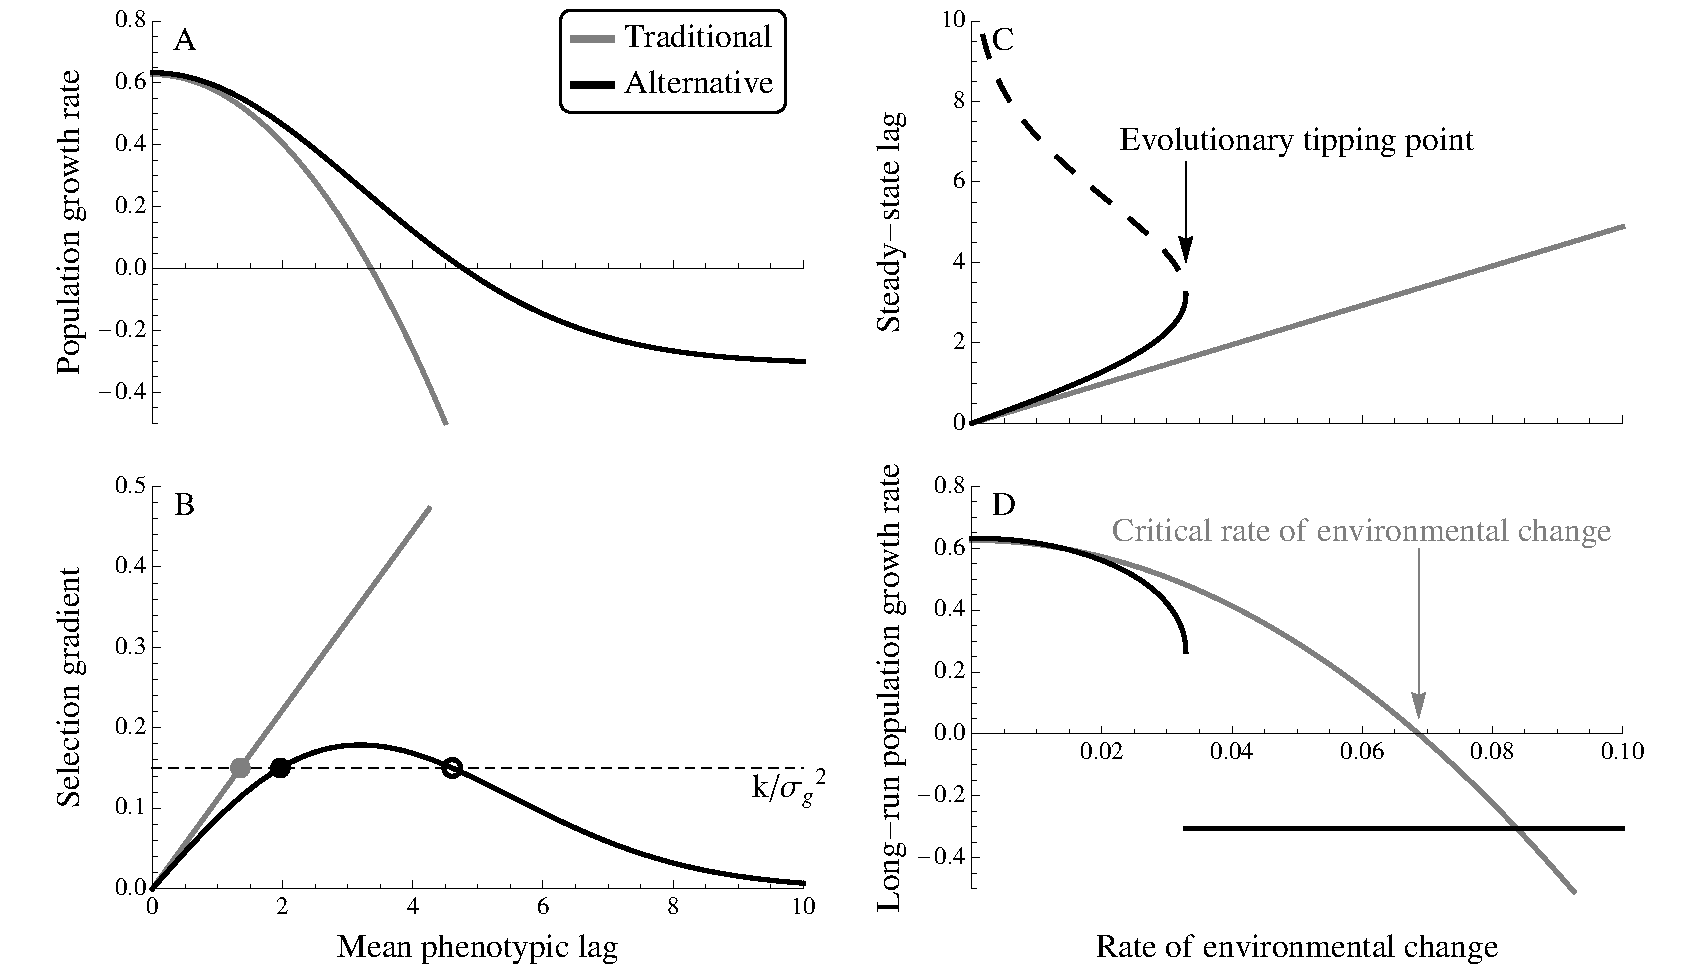
\includegraphics[width=\linewidth]{IMAGES/Didactics}
\caption{
Visual overview of the modelling approach. 
Population mean growth rates, $\bar{r}$, shown in \textbf{A}, are derived by integrating the traditional (\textit{gray}) and alternative (\textit{black}) fitness functions, $r(z)$, over the phenotypic distribution, $p(z)$.
Taking the derivative of mean population growth rate with respect to the mean trait value, $\mathrm{d}\bar{r}/\mathrm{d}\bar{z}$, gives the selection gradients shown in \textbf{B}.
Setting the the rate of evolution equal to the rate of change in the environmental optimum ($\sigma_g^2\mathrm{d}\bar{r}/\mathrm{d}\bar{z} = k$; where the dashed line intersects the solid curves in \textbf{B}) gives the steady-state lags, $\hat{l}$, shown in \textbf{C}.
With the traditional fitness function all steady-state lags are stable (filled circles in \textbf{B} and solid lines in \textbf{C}), while those that are on the decreasing portion of the selection gradient with the alternative fitness function are unstable (open circle in \textbf{B} and dashed lines in \textbf{C}). 
Evaluating population mean growth rate at a stable steady-state lag gives the long-run population growth rates shown in \textbf{D}.
The rate of change that causes a long-run growth rate of zero is the critical rate of environmental change.
Because the long-run population growth rate with an alternative fitness function switches sign without crossing zero at the bifurcation point in \textbf{C}, we call this rate of environmental change an evolutionary tipping point.  
Parameters: $r_m = \log(2)$, $\sigma_w^2 = 9$, $\sigma_e^2 = 1$, $\sigma_g^2\approx0.18$, and $d=1$.
}
\label{SSGrowth}
\end{figure}

%\begin{figure}[!ht]
%\centering
%\includegraphics[width=\linewidth]{IMAGES/SSLagGrowth}
%\caption{
%}
%\label{SSLagGrowth}
%\end{figure}

%\begin{figure}[!ht]
%\centering
%\includegraphics[width=0.75\linewidth]{IMAGES/TradSteadyStateGrowthRate}\\
%\includegraphics[width=0.75\linewidth]{IMAGES/AltSteadyStateGrowthRate}
%\caption{
%}
%\label{SSGrowth}
%\end{figure}

%\begin{figure}[!ht]
%\centering
%\includegraphics[width=0.45\linewidth]{IMAGES/TradModerateSummary}
%\includegraphics[width=0.45\linewidth]{IMAGES/AltModerateSummary}
%\caption{
%moderate selection; all time points
%}
%\label{ModerateSummary}
%\end{figure}

\begin{figure}[!ht]
\centering
%\includegraphics[width=0.45\linewidth]{IMAGES/TradModerateSummaryLast}
%\includegraphics[width=0.45\linewidth]{IMAGES/TradSummaryLastLots}
%\includegraphics[width=0.45\linewidth]{IMAGES/TradSummaryMeanLots}
%\includegraphics[width=0.45\linewidth]{IMAGES/TradSummaryLastLarge}
%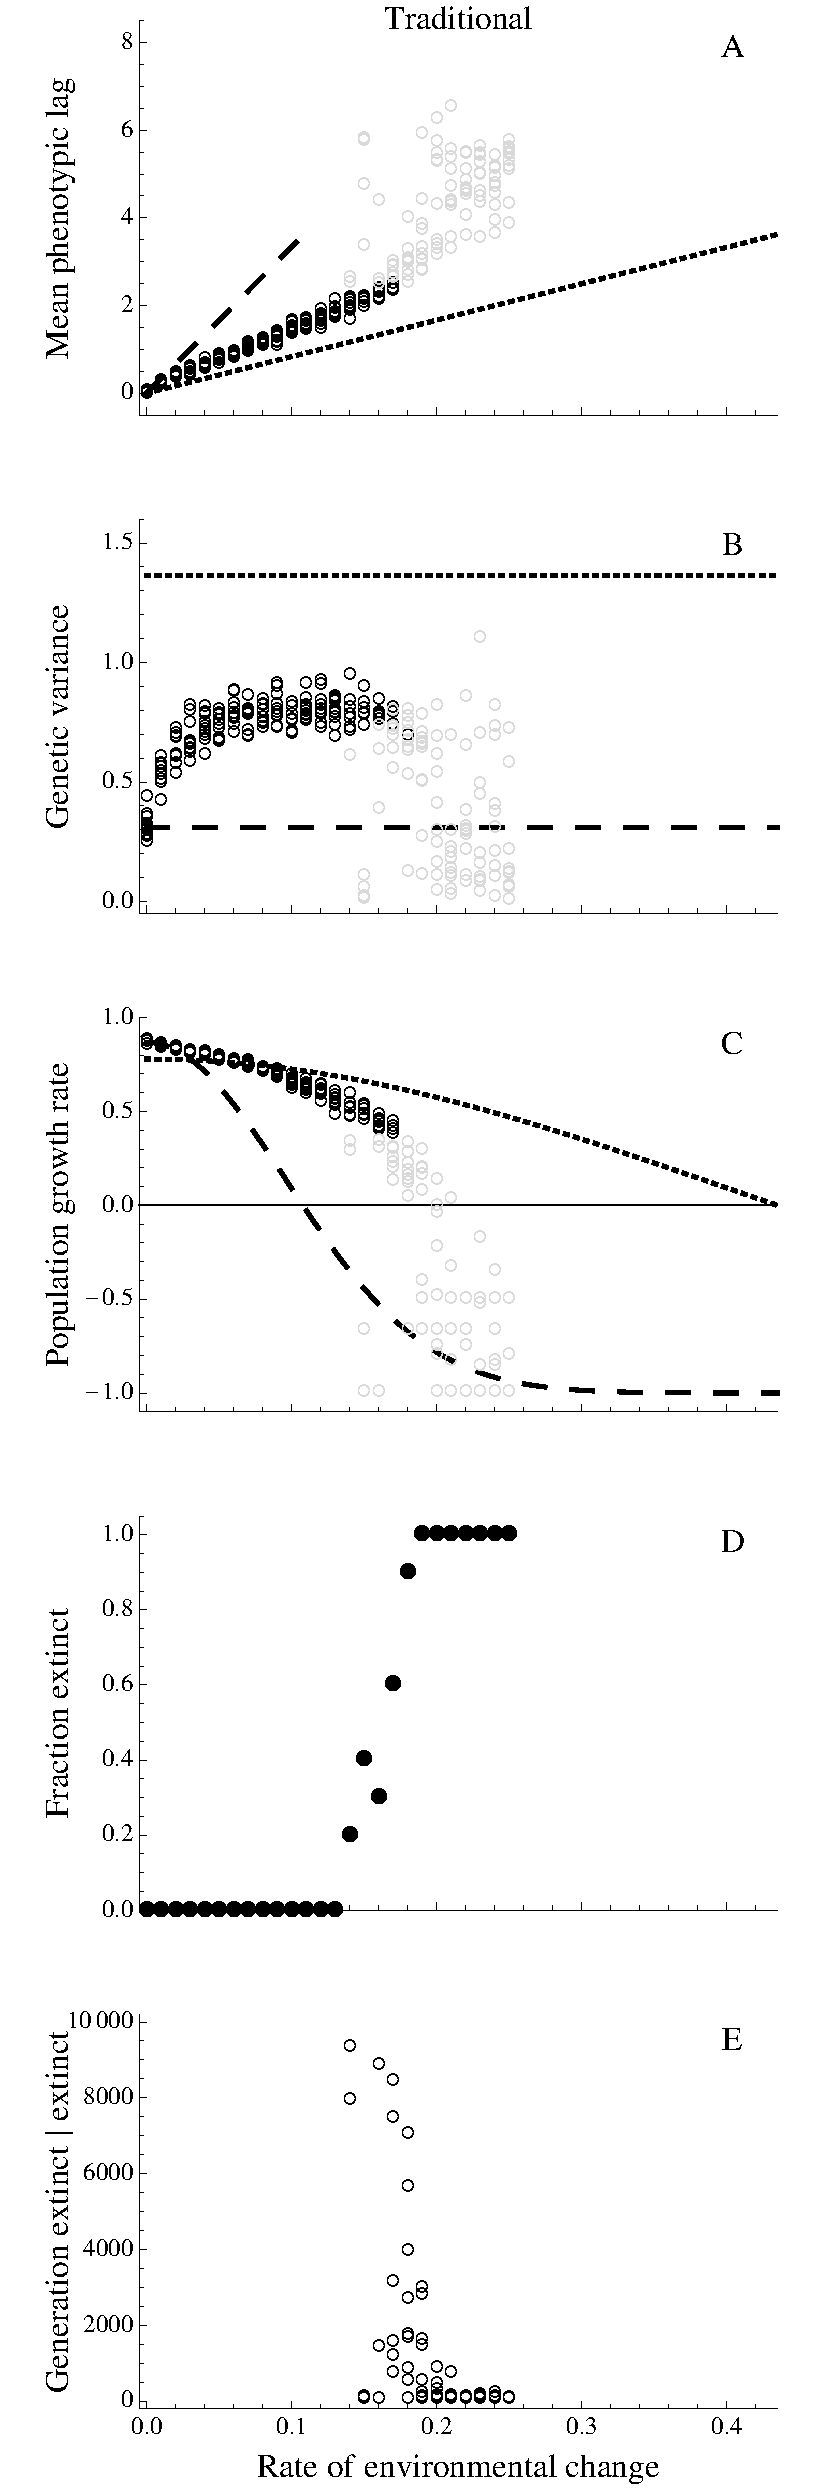
\includegraphics[width=0.45\linewidth]{IMAGES/TradSummaryMeanLargeBurn}
%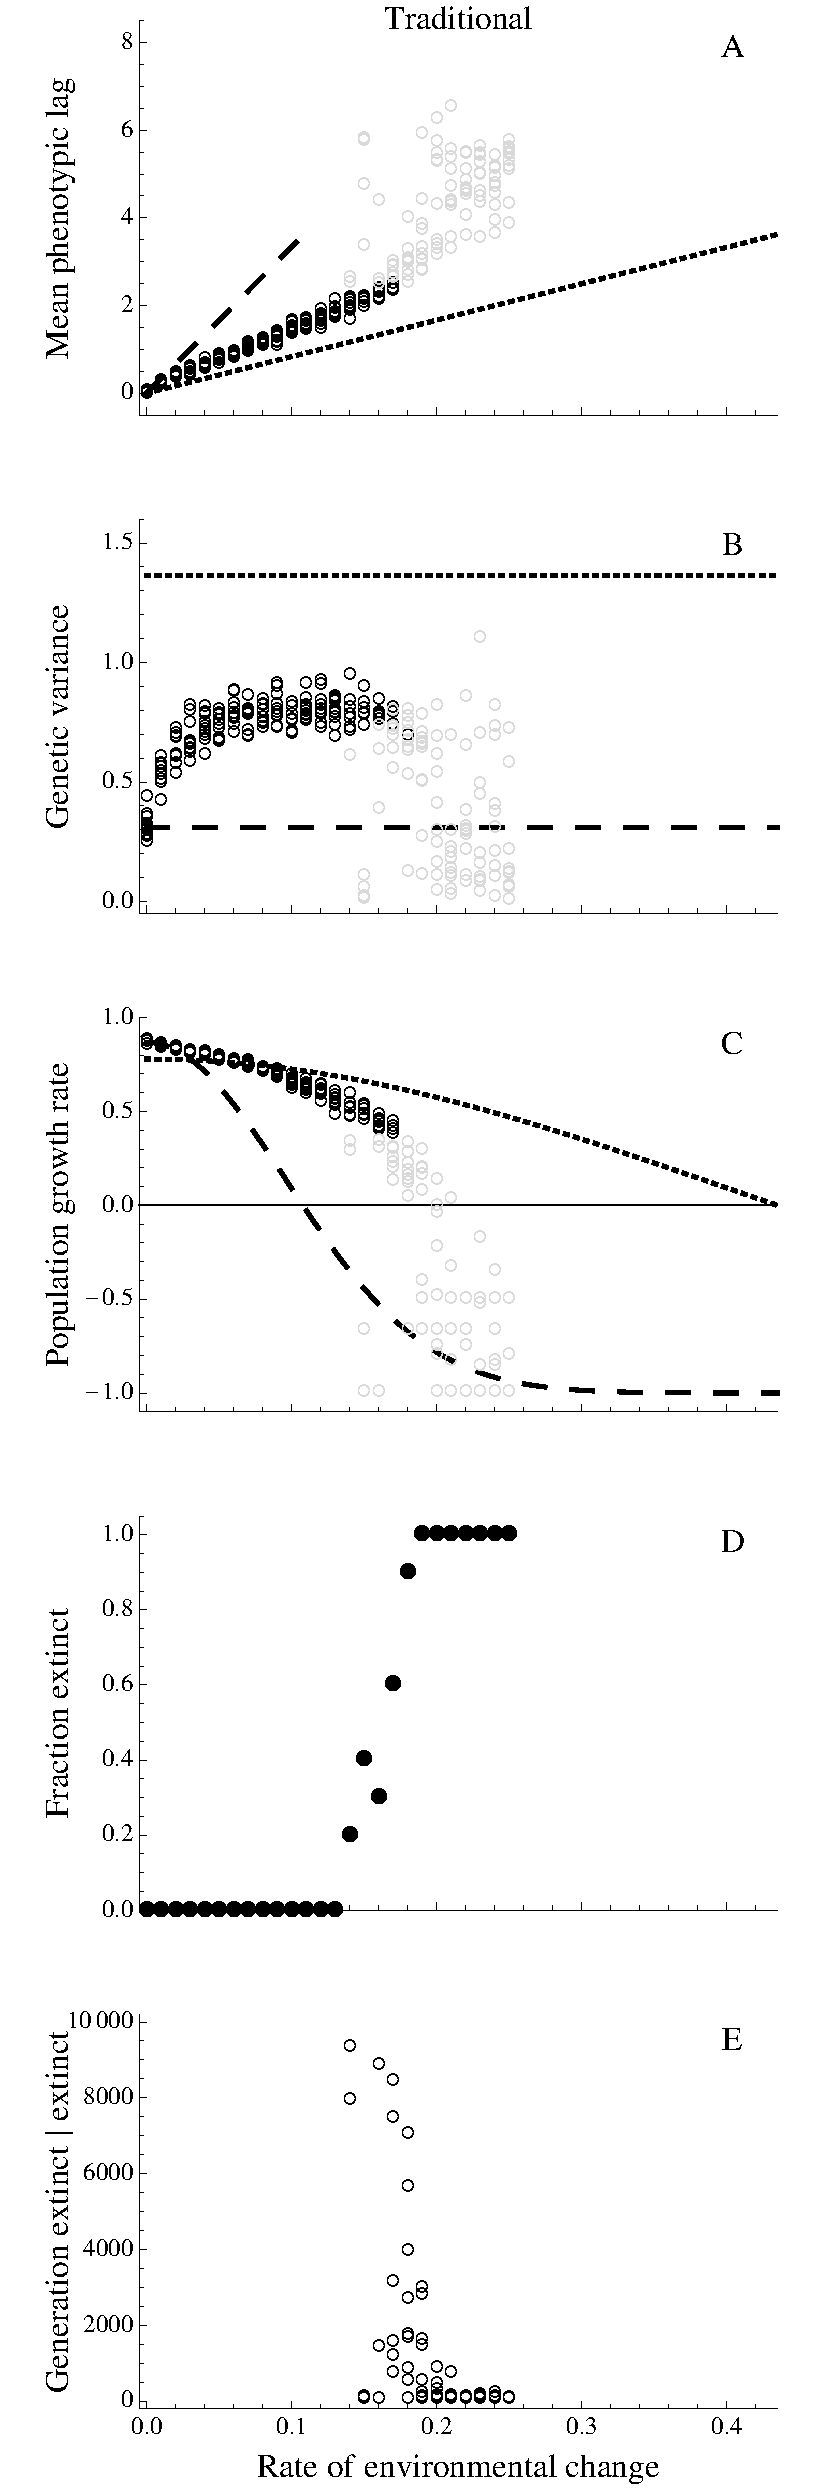
\includegraphics[width=0.45\linewidth]{IMAGES/TradSummaryMeanLargeBurn}
%\includegraphics[width=0.45\linewidth]{IMAGES/TradSummaryLastLargeBurn}
%
%\includegraphics[width=0.45\linewidth]{IMAGES/AltModerateSummaryLast}
%\includegraphics[width=0.45\linewidth]{IMAGES/AltSummaryLastLots}
%\includegraphics[width=0.45\linewidth]{IMAGES/AltSummaryMeanLots}
%\includegraphics[width=0.45\linewidth]{IMAGES/AltSummaryLastLarge}
%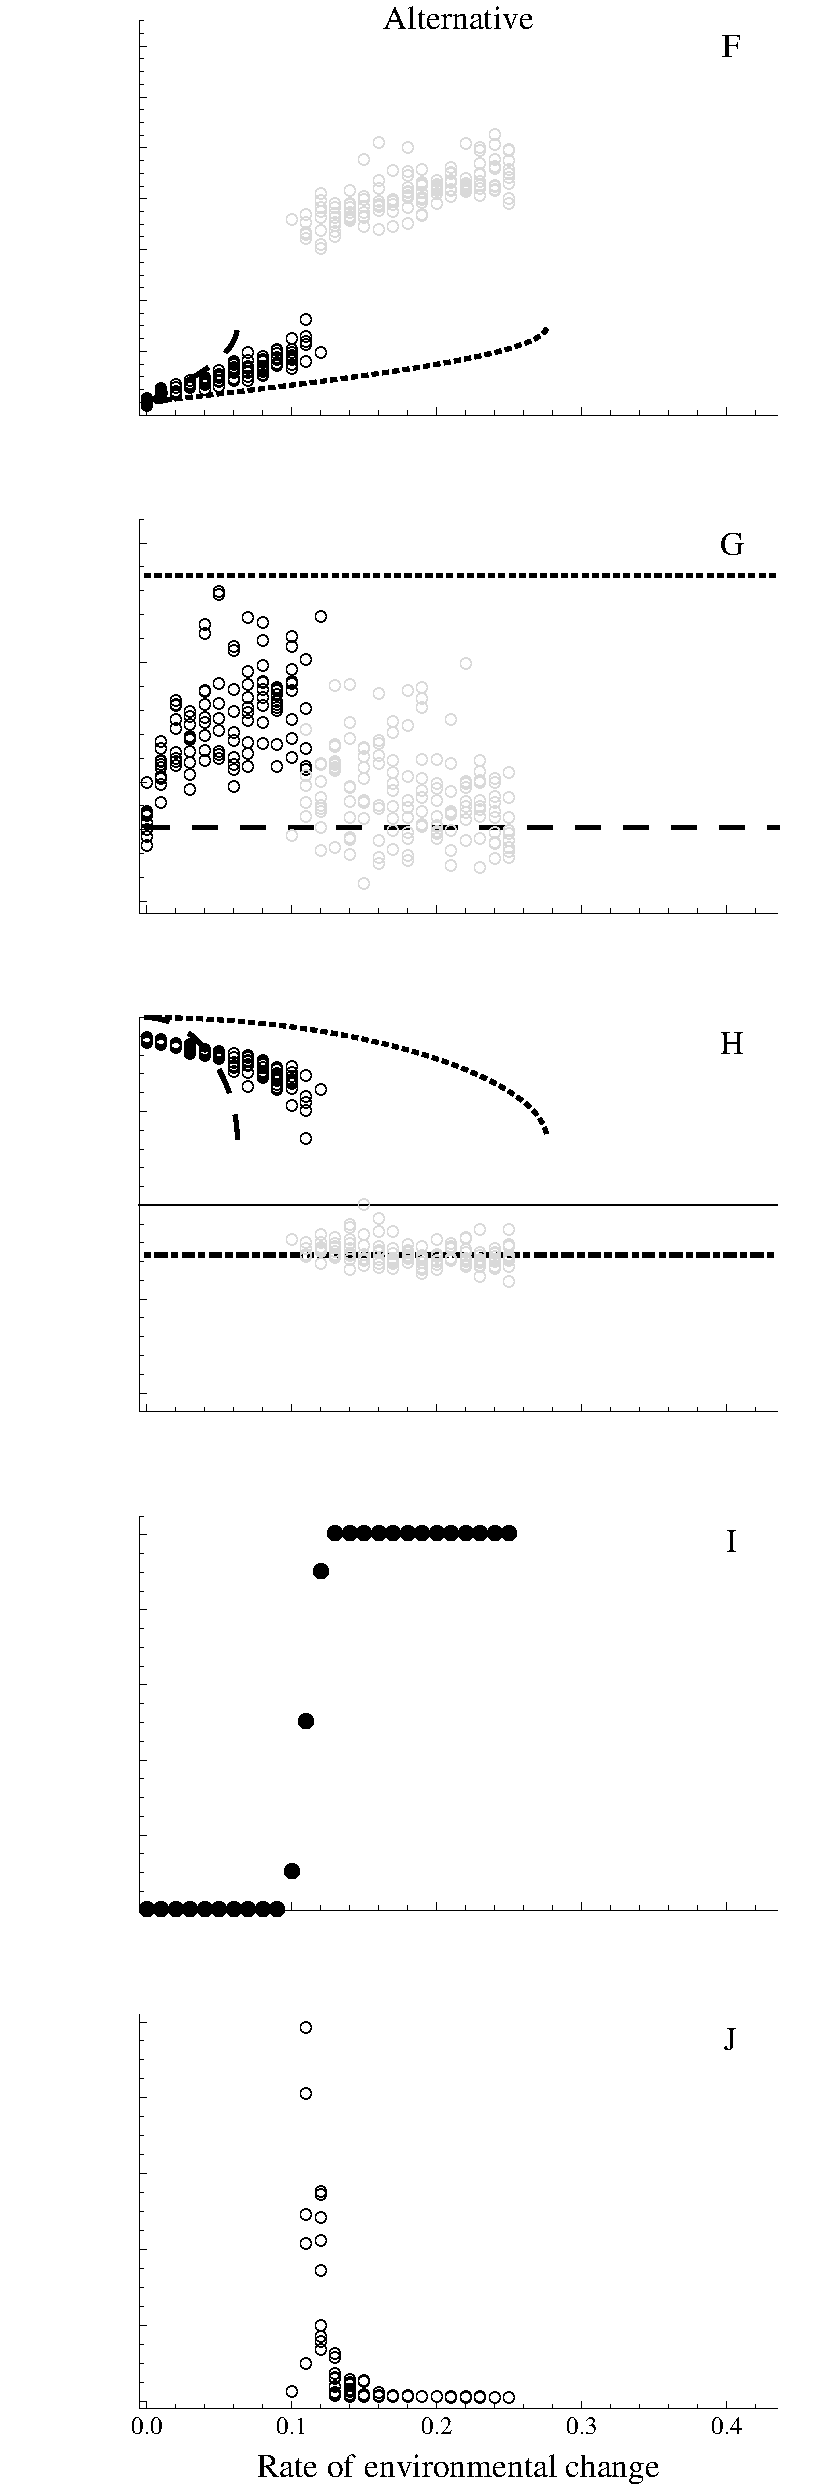
\includegraphics[width=0.45\linewidth]{IMAGES/AltSummaryMeanLargeBurn}
\caption{
Discrete-time, individual-based simulation results with traditional (\textbf{A}-\textbf{E}) and alternative (\textbf{F}-\textbf{J}) fitness functions.
In discrete time the traditional fitness function is $W(z) = \exp\left[ -(\theta - z)^2 / (2\sigma_w^2) \right]$ \citep[][equation 1]{Burger1995} and the alternative fitness function is $W^*(z) = \exp\left[ d(W(z) - 1)\right]$.
``Population growth rate" is the number of offspring surviving viability selection (before density-dependence) divided by the number of parents, minus one. 
``Fraction extinct" is the number of replicates that go extinct before the end of the simulation (generation 11,000).
%Circles and error bars give means $\pm$ 1.96 times the standard error using the last recorded time point only, measured across 10 replicates (\textbf{A},\textbf{B},\textbf{F},\textbf{G} average over only those replicates that did not go extinct; \textbf{E},\textbf{J} average over only those replicates that did go extinct).
In \textbf{A}-\textbf{C} and \textbf{F}-\textbf{H}, circles give mean values over the last 10 recorded time points (every 100 generations) for each replicate simulation (10 for each rate of environmental change), or over all recorded time points since the burn-in if less than 10 time points since the burn-in.
Gray circles are replicates that went extinct before the end of the simulation.  
%``Generation extinct $|$ extinct" uses data from only those replicates that went extinct.     
Broken curves in \textbf{A}-\textbf{C}, and \textbf{F}-\textbf{H} give analytic results using the stochastic-house-of-cards (dashed) and neutral (dotted) approximations for genetic variance \citep[equations 14 and 15 in][]{Burger1995}.
%In \textbf{C} and \textbf{H}, the horizontal line gives a population growth rate of replacement.
Paremeters as in \cite{Burger1995}: $B = 2$, $\sigma_w^2 = 9$, $\sigma_e^2 = 1$, $K=512$, $\mu = 2\times10^{-4}$, $\alpha^2 = 0.05$, $n=50$, and $d=1$.
}
\label{ModerateSummaryLast}
\end{figure}

\begin{figure}[!ht]
\centering
%\includegraphics[width=0.45\linewidth]{IMAGES/TradModerateEarlyWarning}
%\includegraphics[width=0.45\linewidth]{IMAGES/AltModerateEarlyWarning}
%\includegraphics[width=0.45\linewidth]{IMAGES/TradLagGrowthTimeSeries}
%\includegraphics[width=0.45\linewidth]{IMAGES/AltLagGrowthTimeSeries}\\
%\includegraphics[width=0.45\linewidth]{IMAGES/TradVarianceTimeSeries}
%\includegraphics[width=0.45\linewidth]{IMAGES/AltVarianceTimeSeries}\\
%\includegraphics[width=0.45\linewidth]{IMAGES/TradAutoCorrTimeSeries}
%\includegraphics[width=0.45\linewidth]{IMAGES/AltAutoCorrTimeSeries}\\
%\includegraphics[width=0.45\linewidth]{IMAGES/TauVariance}
%\includegraphics[width=0.45\linewidth]{IMAGES/TauAutocorrelation}
%\includegraphics[trim={5cm 9cm 5cm 4.5cm},clip,width=\linewidth]{IMAGES/Figure3}
%\includegraphics[width=\linewidth]{IMAGES/EarlyWarningSigns.eps}
%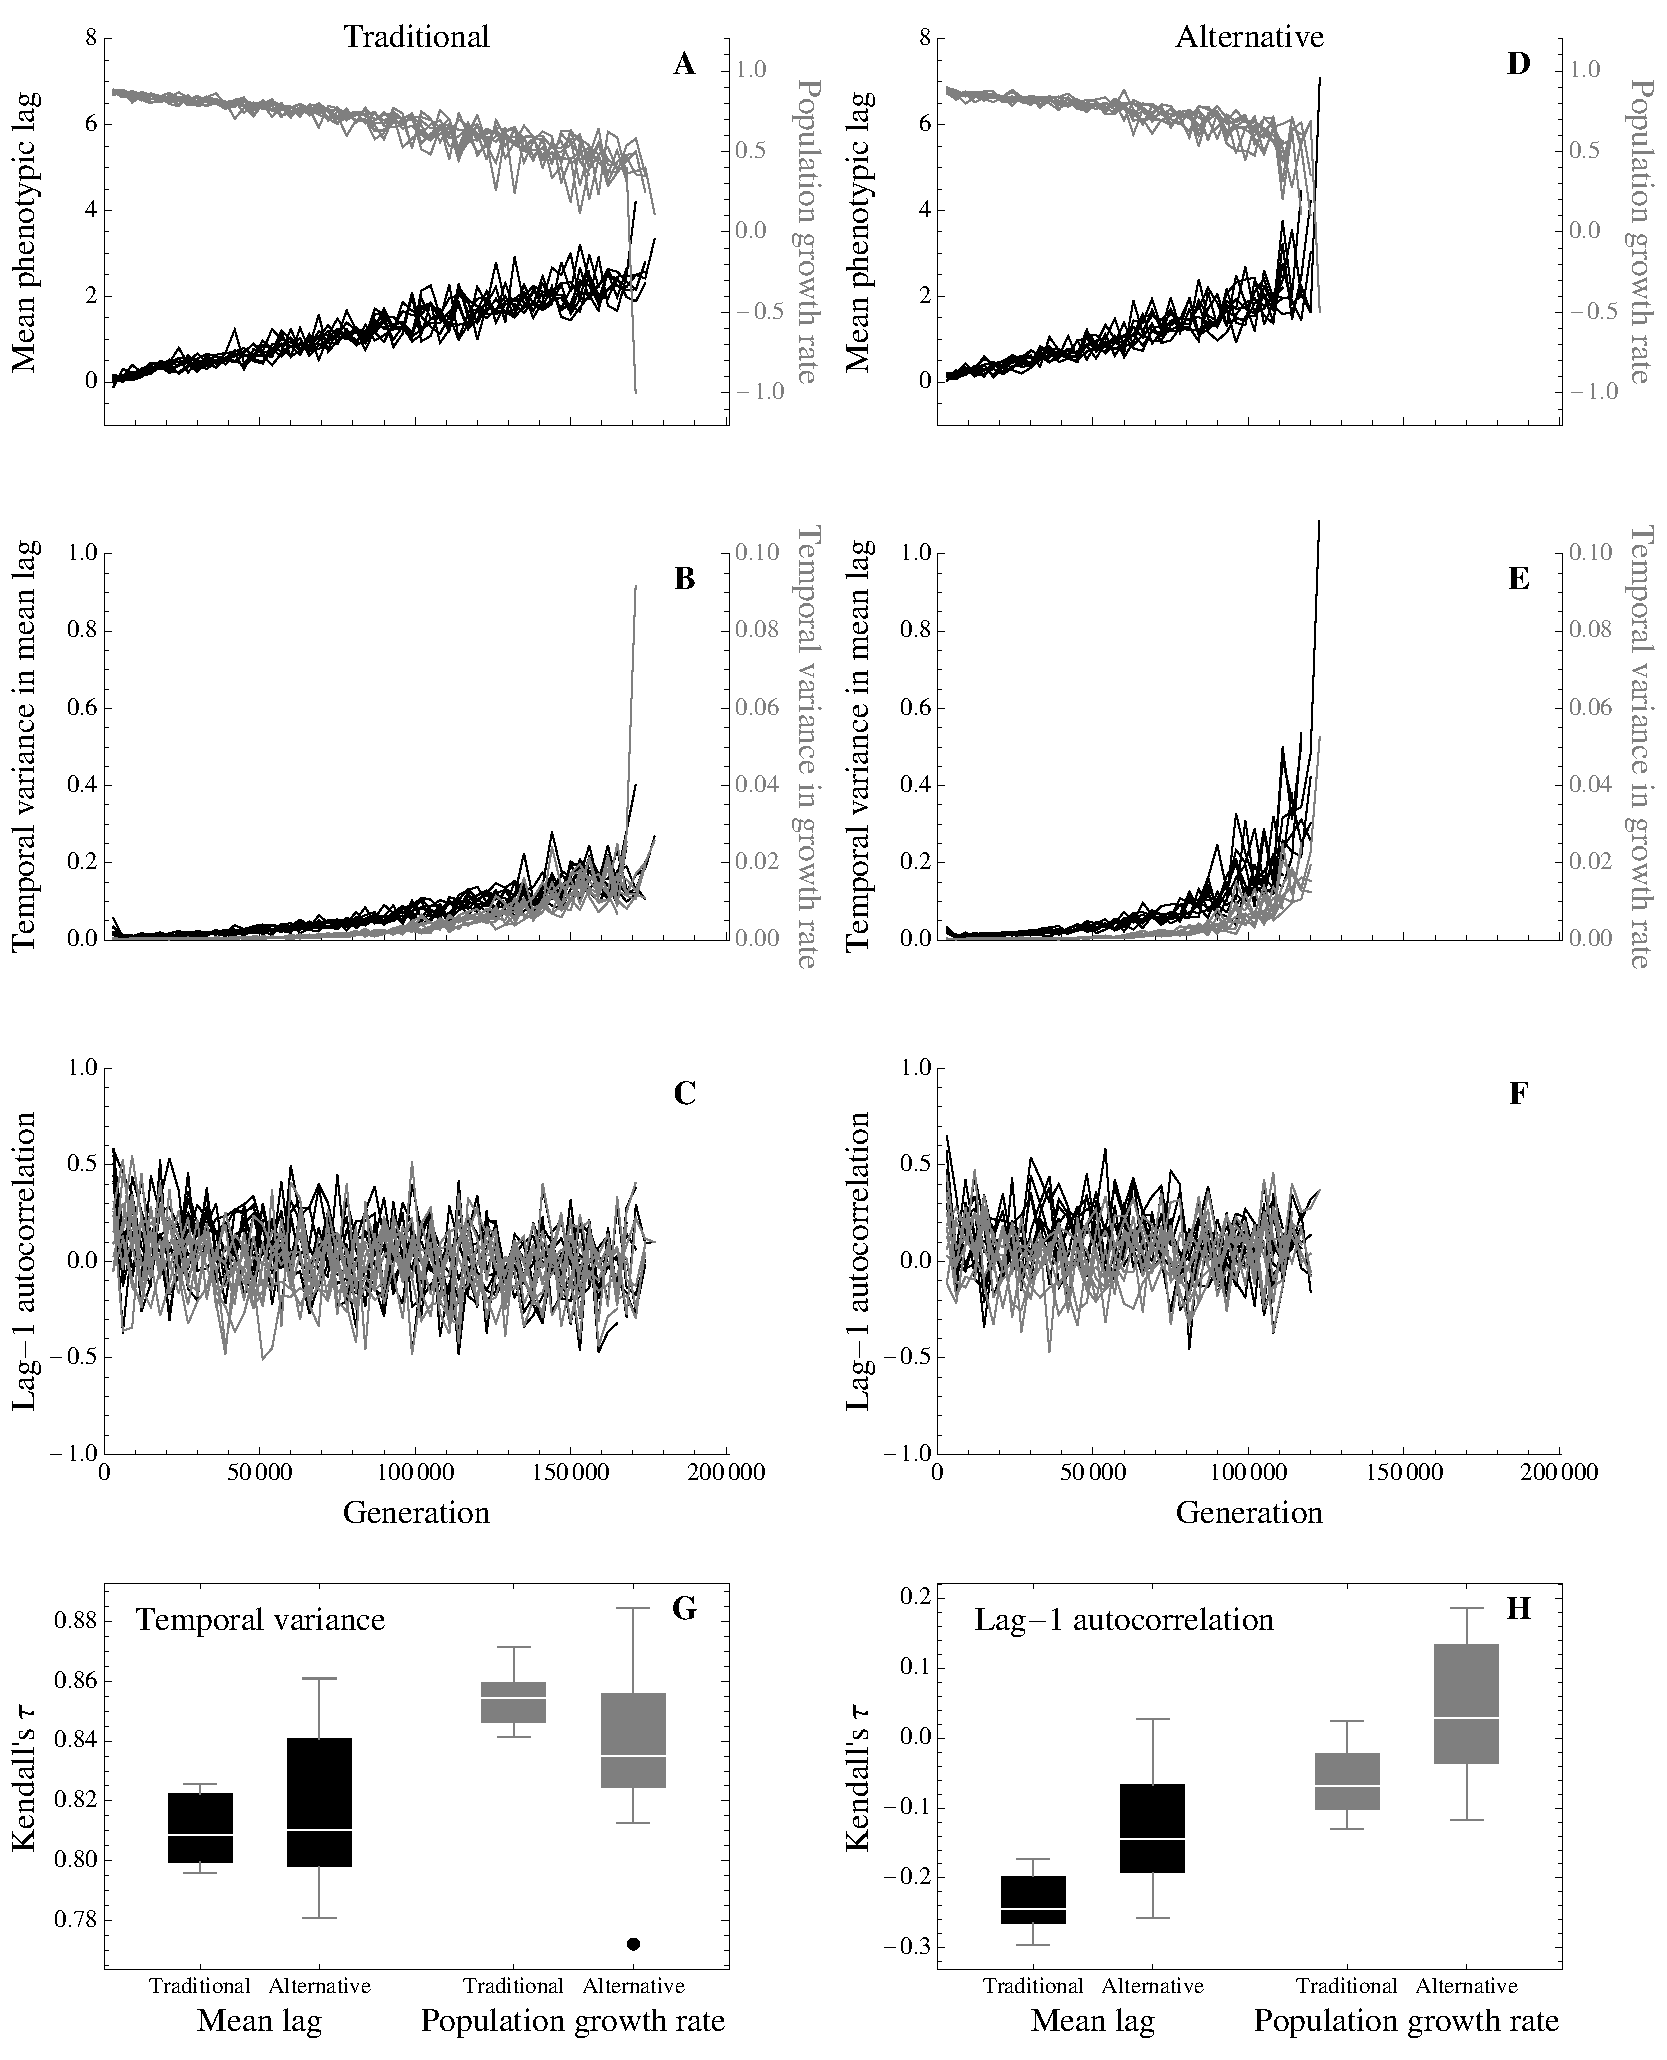
\includegraphics[width=\linewidth]{IMAGES/EarlyWarningSignsLarge-eps-converted-to.pdf}
\caption{
Generic early-warning signs of tipping points.
%Data from the same simulations as shown in Figure \ref{ModerateSummaryLast}.
%Circles and error bars give means $\pm$ 1.96 times the standard error across those replicates which did not go extinct.
%The first 5000 of 10000 generations were discarded as burn-in.
%(\textbf{A, C}) Lag-1 autocorrelation in mean phenotypic lag (black) and population growth rate (gray) over time. 
%(\textbf{B, D}) Coefficient of variation in mean phenotypic lag (black) and population growth rate (gray) over time.
Here the rate of environmental change, $k$, gradually increases from 0 by $10^{-6}$ phenotypic units every generation, eventually causing extinction.
With the traditional fitness function (\textbf{A}-\textbf{C}) there is no saddle-node bifurcation and extinction occurs as the rate of environmental change approaches $k=0.175$, as in Figure \ref{ModerateSummaryLast}.
On the other hand, with the alternative fitness function (\textbf{D}-\textbf{F}) there is a saddle-node bifurcation and extinction is caused by an evolutionary tipping point near $k = 0.125$, as in Figure \ref{ModerateSummaryLast}.
Nevertheless, in both cases the temporal variance in mean phenotypic lag (\textit{black}) and population growth rate (\textit{gray}) tend to increase (\textbf{B},\textbf{E}) and Kendall rank correlation coefficients, $\tau$, do not differ significantly between the two fitness functions (\textbf{G}; details in text). %, although the increase in the variance of mean phenotypic lag is perhaps most dramatic near the saddle-node bifurcation.
\textbf{C} and \textbf{F} show the dynamics of lag-1 autocorrelation in mean phenotypic lag and population growth rate for both fitness functions, and the Kendall rank correlation coefficients (\textbf{H}) indicate that a consistent increase in the lag-1 autocorrelation of population growth rate may be the best predictor of an approaching evolutionary tipping point for this set of parameters (details in text).
Shown are ten replicate simulations for each fitness function, with parameters as in Figure \ref{ModerateSummaryLast}.
Variance and lag-1 autocorrelation are measured for each replicate separately, using non-intersecting windows of 30 consecutively recorded time points, each 100 generations apart.
}
\label{ModerateWarnings}
\end{figure}

\begin{figure}[!ht]
\centering
%\includegraphics[width=0.45\linewidth]{IMAGES/TradHysteresisSnapshot}
%\includegraphics[width=0.45\linewidth]{IMAGES/AltHysteresisSnapshot}
%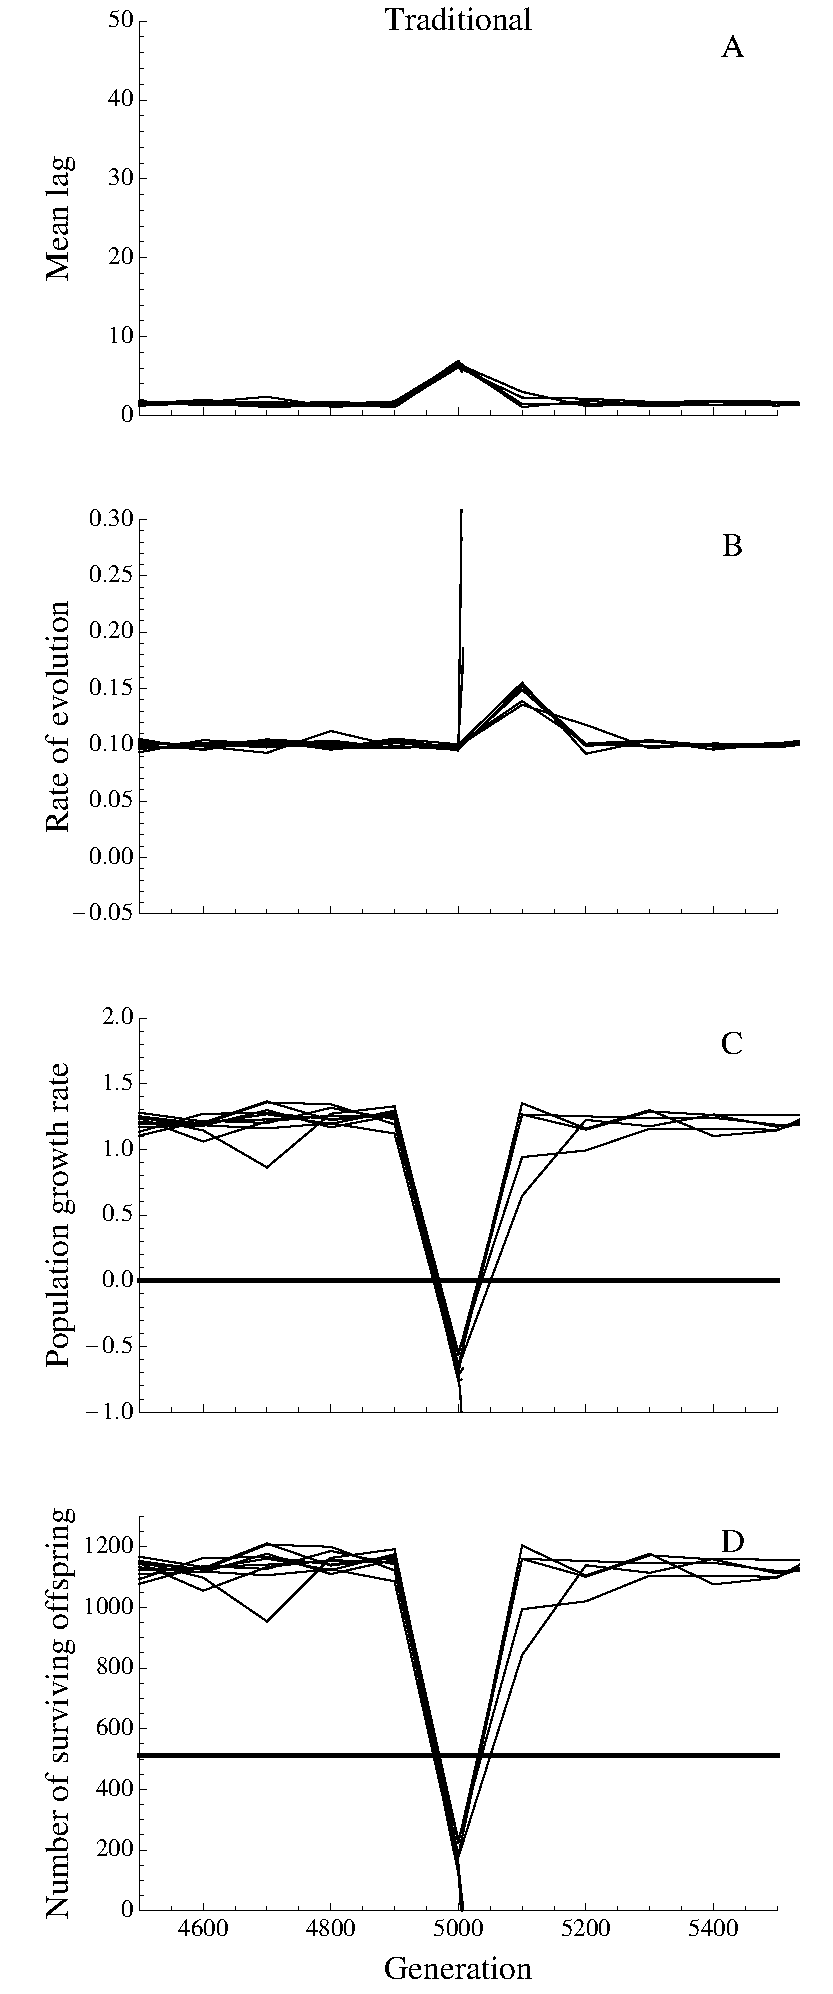
\includegraphics[width=0.45\linewidth]{IMAGES/TradHysteresisSnapshotLarge}
%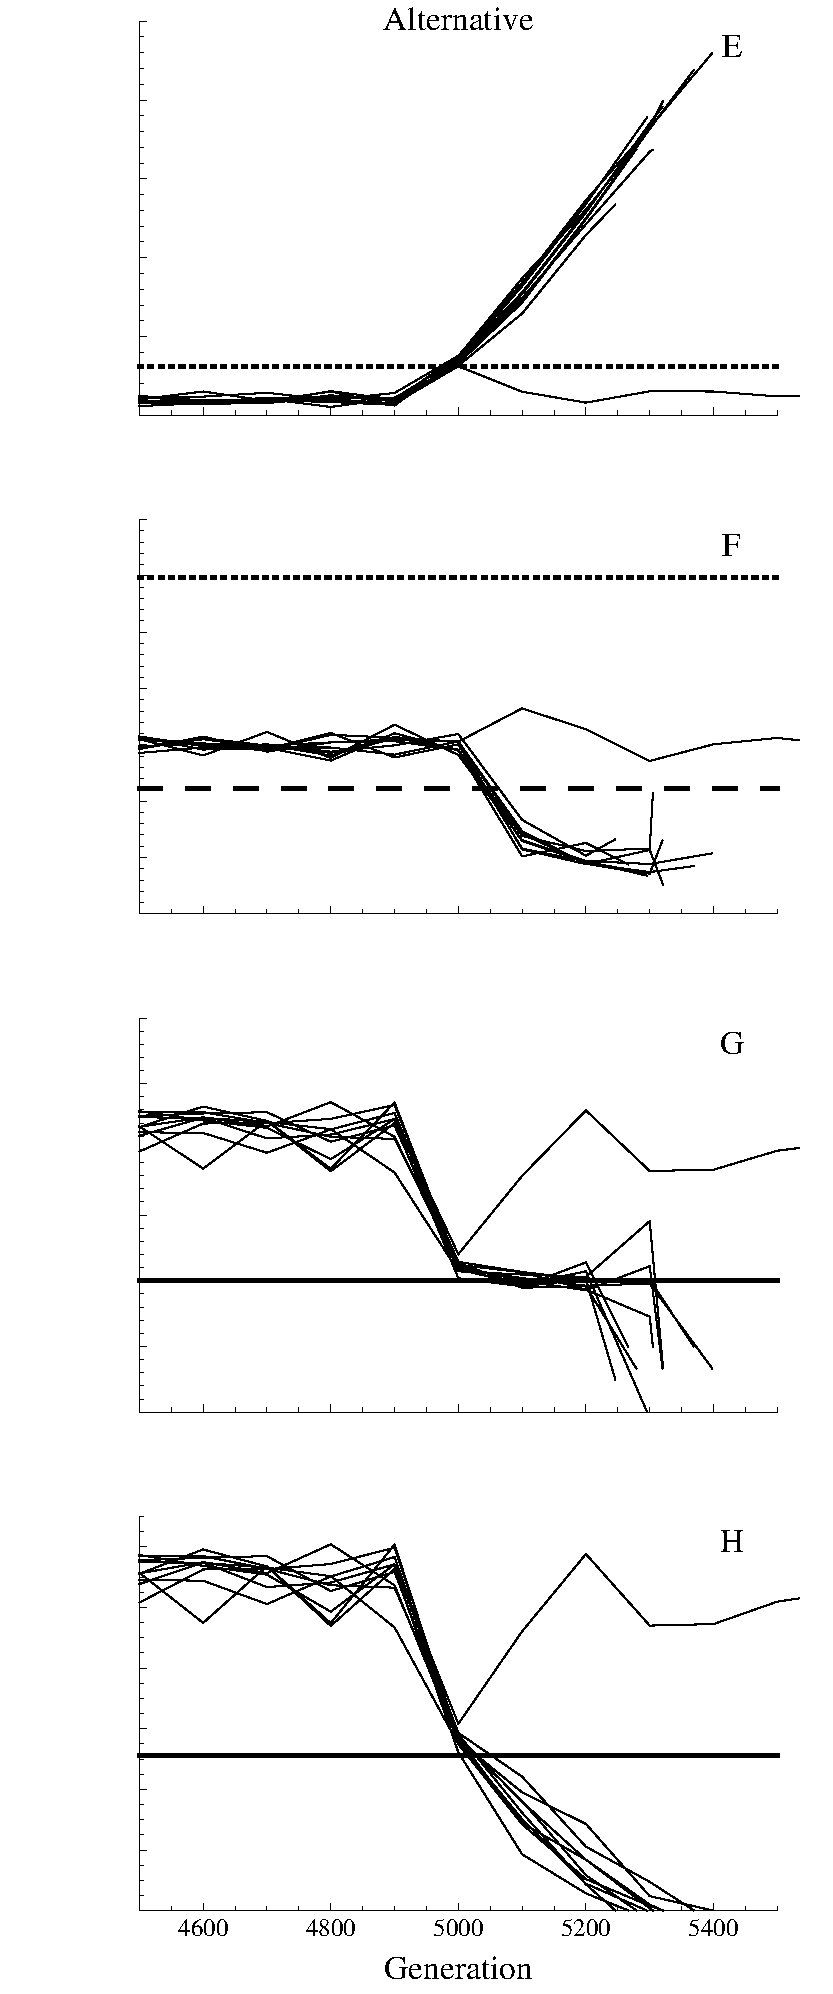
\includegraphics[width=0.45\linewidth]{IMAGES/AltHysteresisSnapshotLarge}
\caption{
Evolutionary hysteresis prevents evolutionary rescue and creates an extinction debt.
Here the optimum trait value increases gradually ($k=0.1$), experiences a sudden jump (5 phenotypic units) at generation 5000, and from there continues to increase at the gradual rate ($k=0.1$).  
With the traditional fitness function (\textbf{A}-\textbf{D}), the sudden increase in mean lag at generation 5000 causes an increase in the strength of selection and hence in the rate of evolution, rescuing populations from extinction.
With the alternative fitness function (\textbf{E}-\textbf{F}), the mean lag increases to values that are often just beyond the basin of attraction of the steady-state lag at $k=0.1$ (dotted line in \textbf{E}, using the neutral approximation for genetic variance; $k=0.1$ is beyond the tipping point with the stochastic-house-of-cards approximation for genetic variance).
(\textbf{F}) The rate of evolution then declines (except in one lucky replicate that does not escape the basin of attraction), causing further increases in the mean lag, which further decreases the rate of evolution, and so on, leading to an apparent existential crisis.
Broken lines show the maximum rate of evolution using the neutral (dotted) and stochastic-house-of-cards (dashed) approximations for genetic variance.
(\textbf{G}) The ever increasing mean lag lowers the population mean growth rate, eventually reaching values below replacement (horizontal line).
(\textbf{H}) This drop in population growth rates ultimately, some $\sim$300 generations later, results in extinction.
The horizontal line is the maximum number of parents, $K$.
Here the fitness functions (see Figure \ref{ModerateSummaryLast}) are multiplied by $(1-d')$, the probability that an optimally adapted individual survives viability selection.
This generalization gives more flexibility in minimum growth rate without affecting the strength of selection.
Parameters as in Figure \ref{ModerateSummaryLast}, except $B=3$ and $d'=0.1$.
}
\label{HysteresisSnapshot}
\end{figure}

%\appendix
%\newpage
%%%%%%%%%%%%%%
%\section*{Appendix: Simulation methods}
%\label{SimApp}
%%%%%%%%%%%%%%
%
%Individual-based simulations followed a Gillespie algorithm (\citealt{Gillespie1977}).
%Populations were represented by a vector of trait values (one entry for each individual), and were initiated with a vector of length $N_0=100$ with each entry pulled from a random normal distribution with mean 0 and variance $2 \alpha^2$ (the predicted equilibrium phenotypic variance).
%
%For each iteration 
%(1) the propensities for each type of reaction (birth, death) were calculated for each individual, 
%(2) the propensities were summed to give the total propensity, $a_0$, 
%(3) time was increased by $\tau = - \mathrm{log}(r_1)/a_0$, where $r_1$ is a random uniform number in $[0,1)$,
%(4) a particular reaction was chosen by giving a reaction with propensity $a_i$ a probability of occurrence $a_i/a_0$ and choosing a random uniform number in $[0,1)$, and
%(5) the reaction occurred and abundances were updated accordingly.
%When an individual was chosen to reproduce, a second individual was chosen randomly as the mate (possibly the same individual), and the offspring inherited the average of the two parental trait values plus a random normal effect with mean 0 and variance $\alpha^2$.
%To reduce simulation times, if there were greater than $K$ individuals after an iteration we randomly selected $K$ survivors before updating.
%
%The abundances and the mean and variance of the trait distributions were recorded every $outputFreq$ iterations.
%Simulations ended when the population went extinct or the final time was reached, $t \geq maxTime$.
%The means of the final $recsteps$ recorded values were used to estimate the steady-state lag, equilibrium population density, and equilibrium phenotypic variance of a replicate.
%
%All simulations were implemented in \texttt{Python} (version 2.7.3; http://www.python.org/) on the WestGrid cluster. 
%An example script is provided in the supplementary online material.
%%The scripts and results are freely available online (link from journal office). %(https://github.com/mmosmond/TIPPINGPOINT.git).


\end{document}
